%% BioMed_Central_Tex_Template_v1.06
%%                                      %
%  bmc_article.tex            ver: 1.06 %
%                                       %

%%IMPORTANT: do not delete the first line of this template
%%It must be present to enable the BMC Submission system to
%%recognise this template!!

%%%%%%%%%%%%%%%%%%%%%%%%%%%%%%%%%%%%%%%%%
%%                                     %%
%%  LaTeX template for BioMed Central  %%
%%     journal article submissions     %%
%%                                     %%
%%          <8 June 2012>              %%
%%                                     %%
%%                                     %%
%%%%%%%%%%%%%%%%%%%%%%%%%%%%%%%%%%%%%%%%%

%%%%%%%%%%%%%%%%%%%%%%%%%%%%%%%%%%%%%%%%%%%%%%%%%%%%%%%%%%%%%%%%%%%%%
%%                                                                 %%
%% For instructions on how to fill out this Tex template           %%
%% document please refer to Readme.html and the instructions for   %%
%% authors page on the biomed central website                      %%
%% https://www.biomedcentral.com/getpublished                      %%
%%                                                                 %%
%% Please do not use \input{...} to include other tex files.       %%
%% Submit your LaTeX manuscript as one .tex document.              %%
%%                                                                 %%
%% All additional figures and files should be attached             %%
%% separately and not embedded in the \TeX\ document itself.       %%
%%                                                                 %%
%% BioMed Central currently use the MikTex distribution of         %%
%% TeX for Windows) of TeX and LaTeX.  This is available from      %%
%% https://miktex.org/                                             %%
%%                                                                 %%
%%%%%%%%%%%%%%%%%%%%%%%%%%%%%%%%%%%%%%%%%%%%%%%%%%%%%%%%%%%%%%%%%%%%%

%%% additional documentclass options:
%  [doublespacing]
%  [linenumbers]   - put the line numbers on margins

%%% loading packages, author definitions

%\documentclass[twocolumn]{bmcart}% uncomment this for twocolumn layout and comment line below
\documentclass{bmcart}

%%% Load packages
\usepackage{amsthm,amsmath}
% \RequirePackage[numbers]{natbib}
% \RequirePackage[authoryear]{natbib}% uncomment this for author-year bibliography
\RequirePackage{hyperref}
\usepackage[utf8]{inputenc} %unicode support
\usepackage[noadjust]{cite}
\usepackage{amsmath,amssymb,amsfonts}
\usepackage{algorithmic}
\usepackage{graphicx}
\usepackage{textcomp}
\usepackage{xcolor}
\usepackage{array,etoolbox,multirow}
\usepackage{float}
\usepackage{caption} 
\usepackage{multirow}
\usepackage{enumitem}
\usepackage{lscape}
\usepackage{lineno,hyperref,longtable}
\usepackage[]{mdframed}
\usepackage{titlesec}
\captionsetup[table]{skip=6pt}

\setcounter{secnumdepth}{4}

\titleformat{\paragraph}
{\normalfont\normalsize\itshape}{\theparagraph}{0.3em}{}
\titlespacing*{\paragraph}
{0pt}{1.6ex plus 1ex minus .2ex}{.5ex plus .2ex}

% \usepackage[applemac]{inputenc} %applemac support if unicode package fails
% \usepackage[latin1]{inputenc} %UNIX support if unicode package fails

%%%%%%%%%%%%%%%%%%%%%%%%%%%%%%%%%%%%%%%%%%%%%%%%%
%%                                             %%
%%  If you wish to display your graphics for   %%
%%  your own use using includegraphic or       %%
%%  includegraphics, then comment out the      %%
%%  following two lines of code.               %%
%%  NB: These line *must* be included when     %%
%%  submitting to BMC.                         %%
%%  All figure files must be submitted as      %%
%%  separate graphics through the BMC          %%
%%  submission process, not included in the    %%
%%  submitted article.                         %%
%%                                             %%
%%%%%%%%%%%%%%%%%%%%%%%%%%%%%%%%%%%%%%%%%%%%%%%%%

% \def\includegraphic{}
% \def\includegraphics{}

%%% Put your definitions there:
\startlocaldefs
\endlocaldefs

%%% Begin ...
\begin{document}

%%% Start of article front matter
\begin{frontmatter}

\begin{fmbox}
\dochead{Research}

%%%%%%%%%%%%%%%%%%%%%%%%%%%%%%%%%%%%%%%%%%%%%%
%%                                          %%
%% Enter the title of your article here     %%
%%                                          %%
%%%%%%%%%%%%%%%%%%%%%%%%%%%%%%%%%%%%%%%%%%%%%%

\title{Application of Microservices Patterns to Big Data Systems}

%%%%%%%%%%%%%%%%%%%%%%%%%%%%%%%%%%%%%%%%%%%%%%
%%                                          %%
%% Enter the authors here                   %%
%%                                          %%
%% Specify information, if available,       %%
%% in the form:                             %%
%%   <key>={<id1>,<id2>}                    %%
%%   <key>=                                 %%
%% Comment or delete the keys which are     %%
%% not used. Repeat \author command as much %%
%% as required.                             %%
%%                                          %%
%%%%%%%%%%%%%%%%%%%%%%%%%%%%%%%%%%%%%%%%%%%%%%

\author[
  addressref={aff1},                   % id's of addresses, e.g. {aff1,aff2}
  corref={aff1},                       % id of corresponding address, if any
% noteref={n1},                        % id's of article notes, if any
  email={jane.e.doe@cambridge.co.uk}   % email address
]{\inits{P.A.}\fnm{Pouya} \snm{Ataei}}
\author[
  addressref={aff1,aff2},
  email={john.RS.Smith@cambridge.co.uk}
]{\inits{D.S.}\fnm{Daniel} \snm{Staegemann}}

%%%%%%%%%%%%%%%%%%%%%%%%%%%%%%%%%%%%%%%%%%%%%%
%%                                          %%
%% Enter the authors' addresses here        %%
%%                                          %%
%% Repeat \address commands as much as      %%
%% required.                                %%
%%                                          %%
%%%%%%%%%%%%%%%%%%%%%%%%%%%%%%%%%%%%%%%%%%%%%%

\address[id=aff1]{%                           % unique id
  \orgdiv{Department of Science},             % department, if any
  \orgname{University of Cambridge},          % university, etc
  \city{London},                              % city
  \cny{UK}                                    % country
}
\address[id=aff2]{%
  \orgdiv{Institute of Biology},
  \orgname{National University of Sciences},
  %\street{},
  %\postcode{}
  \city{Kiel},
  \cny{Germany}
}

%%%%%%%%%%%%%%%%%%%%%%%%%%%%%%%%%%%%%%%%%%%%%%
%%                                          %%
%% Enter short notes here                   %%
%%                                          %%
%% Short notes will be after addresses      %%
%% on first page.                           %%
%%                                          %%
%%%%%%%%%%%%%%%%%%%%%%%%%%%%%%%%%%%%%%%%%%%%%%

%\begin{artnotes}
%%\note{Sample of title note}     % note to the article
%\note[id=n1]{Equal contributor} % note, connected to author
%\end{artnotes}

\end{fmbox}% comment this for two column layout

%%%%%%%%%%%%%%%%%%%%%%%%%%%%%%%%%%%%%%%%%%%%%%%
%%                                           %%
%% The Abstract begins here                  %%
%%                                           %%
%% Please refer to the Instructions for      %%
%% authors on https://www.biomedcentral.com/ %%
%% and include the section headings          %%
%% accordingly for your article type.        %%
%%                                           %%
%%%%%%%%%%%%%%%%%%%%%%%%%%%%%%%%%%%%%%%%%%%%%%%

\begin{abstractbox}

\begin{abstract} % abstract
  The panorama of data is ever evolving, and big data has emerged to become one of the most hyped terms in the industry. Today, users are the perpetual producers of data that if gleaned and crunched, will yield game-changing patterns. This has introduced an important shift about the role of data in organizations and many strived to harness to power of this new material. Howbeit, institutionalizing data is not an easy task and requires the absorption of a great deal of complexity. According to the literature, it is estimated that only 13\% of organizations succeeded in delivering on their data strategy. Among the root challenges, big data system development and data architecture are prominent. To this end, this study aims to facilitate data architecture and big data system development by applying well-established patterns of microservices architecture to big data systems. This objective is achieved by two systematic literature reviews, and infusion of results through thematic synthesis. The result of this work is a series of theories that explicates how microservices patterns could be useful for big data systems. These theories are then validated through a semi-structured interview with 7 experts from the industry. The findings emerged from this study indicates that big data architecture can benefit from many principles and patterns of microservices architecture. 
\end{abstract}

%%%%%%%%%%%%%%%%%%%%%%%%%%%%%%%%%%%%%%%%%%%%%%
%%                                          %%
%% The keywords begin here                  %%
%%                                          %%
%% Put each keyword in separate \kwd{}.     %%
%%                                          %%
%%%%%%%%%%%%%%%%%%%%%%%%%%%%%%%%%%%%%%%%%%%%%%

\begin{keyword}
\kwd{big data}
\kwd{microservices}
\kwd{microservices patterns}
\kwd{big data architecture}
\kwd{data architecture}
\kwd{data engineering}
\end{keyword}

% MSC classifications codes, if any
%\begin{keyword}[class=AMS]
%\kwd[Primary ]{}
%\kwd{}
%\kwd[; secondary ]{}
%\end{keyword}

\end{abstractbox}
%
%\end{fmbox}% uncomment this for two column layout

\end{frontmatter}

%%%%%%%%%%%%%%%%%%%%%%%%%%%%%%%%%%%%%%%%%%%%%%%%
%%                                            %%
%% The Main Body begins here                  %%
%%                                            %%
%% Please refer to the instructions for       %%
%% authors on:                                %%
%% https://www.biomedcentral.com/getpublished %%
%% and include the section headings           %%
%% accordingly for your article type.         %%
%%                                            %%
%% See the Results and Discussion section     %%
%% for details on how to create sub-sections  %%
%%                                            %%
%% use \cite{...} to cite references          %%
%%  \cite{koon} and                           %%
%%  \cite{oreg,khar,zvai,xjon,schn,pond}      %%
%%                                            %%
%%%%%%%%%%%%%%%%%%%%%%%%%%%%%%%%%%%%%%%%%%%%%%%%

%%%%%%%%%%%%%%%%%%%%%%%%% start of article main body
% <put your article body there>

%%%%%%%%%%%%%%%%
%% Background %%
%%

\section{Introduction}


Today, we live in a world that produces data at an unprecedented rate. The attention toward these large volume of data has been growing rapidly and many strive to harness the advantages of this new material. Along these lines, academics and practitioners have considered means through which they can incorporate data-driven functions and explore patterns that were otherwise unknown. While the opportunities exist with big data (BD), there are many failed attempts. According to New Vantage Partners report in 2022, only 26.5\% of companies successfully became data-driven \cite{NewVantageSurvey}. Another survey by Databricks highlighted that only 13\% of organizations succeeded in delivering on their data strategy \cite{DataBricksSurvey}. 

Therefore, there is an increasing need for more research on reducing the complexity involved with BD projects. One area with good potential is data architecture. Data architecture allows for a flexible and scalable BD system that can account for emerging requirements. One way to absorb the body of knowledge available on data architecture, can be reference architectures (RAs). By presenting proven ways to solve common implementation challenges on an architectural level, RAs support the development of new systems by offering guidance and orientation.


% Despite the important, there's not enough attention to this space. 



% 

% Though, because there might have been new propositions since then, an update might be necessary.

Another concept that has the potential to help with development of BD systems is the use of microservices (MS) architecture. MS architecture allows for division of complex applications into small, independent, and highly scalable parts and, therefore, increase maintainability and allows for a more flexible implementation \cite{Richardson.2022}. Nevertheless, design and development of MS is sophisticated, since heterogenous services have to interact with each other to achieve the overall goal of the system. One way to reduce that complexity is the use of patterns. Comparable to RAs, they are proven artifacts on how certain problems could be solved. In the realm of MS, there are numerous patters that can be utilized, depending on the desired properties of the developed system. Despite the potential of RAs and MS architectures to solve some of complexities of BD development, to our knowledge, there is no study that properly bridge these two concepts. 

% While practitioners in the domain of MS architecture seem to benefit from many well-established practices, data engineering does not seem be absorbing many of these concepts. 

To this end, this study aims to explore the application of MS patterns to BD systems, in aspiration to solve some of the complexities of BD system development. For this purpose, the result of two distinct systematic literature reviews (SLRs) are combined. The first SLR is conducted as part of this study to collect all MS patterns in the body of knowledge. The results of these SLRs are collected, captured and combined through thematic synthesis. As a result, various design theories are generated and validated through a semi-structured interview. The second SLR is done by \cite{ataei2022state} to find all BD reference architectures (RAs) available in the body of knowledge and to point out architectural constructus and limitations. 


% For this purpose, following this introduction as well as a background section and a description of the followed methodology, the literature review on BD reference architectures (Ataei and Litchfield 2020) is updated up until June 2022. Further, a thorough literature review on microservice patterns is conducted, complying with the Prisma guidelines (Page et al. 2021). Subsequently, the identified patterns are matched to the updated list of BD reference architectures. Finally, the results are discussed and a conclusion is given.

The contribution of this study, is thereby threefold: 1) it provides an updated synopsis of the existing BD reference architectures, 2) it assembles an overview of relevant microservice patterns and, most importantly, 3) it creates a connection between the two to facilitate BD system development and architecture.


% Daniel
\section{Related Work}

To the best of our knowledge, there is no study in academia that has shared the same goal as our study. Laigner et al. \cite{laigner2020monolithic} applied an action research and reported on experience of  replacing a legacy BDS with a microservice-based event-driven system. This study is not a systematic review and aims to create contextualized theory in a controlled environment. In another effort,  Zhelev et al. \cite{zhelev2019using} described why event-driven architectures could be a good alternative to monolithic architectures. This study does not follow any clear methodology, and seems to contribute only in terms of untested theory.

Staegemann et al \cite{staegemann2021examining} examined the interplay between BD and MS by conducting a bibliometric review. This study aims to provide with a general picture of the topic, and does not aim to explore MS patterns and their relationship to BD systems.  While the problem of BD system development has been approached through a RA that absorbs some of the concepts from MS architectures as seen in Phi \cite{Phi} and Neomycelia \cite{ataei2021neomycelia}, there is no study that aimed to apply MS patterns to BD systems through a systematic methodology.


% % Daniel
\section{Methodology}

Since the goal of this study is to map BD architectures and microservice patterns, it is consequently mandatory to get a comprehensive overview over both domains. For this purpose, it was decided to conduct two systematic literature reviews (SLR), one for each domain. Both SLRs are conducted following the guidelines presented in Kitchenham et al. \cite{Kitchenham.2004} and Page et al. \cite{Page.2021} on Preferred Reporting Items for Systematic Reviews and Meta-Analyses (PRISMA). The former was used because of its clear instructions on critically appraising evidence for validity, impact and applicability in software engineering and the latter was used because it's a comprehensive and well-established methodology for increasing systematicity, transparency, and prevention of bias. To synthesize our findings, thematic synthesis proposed by Cruzes and Dyba was applied \cite{Cruzes.2011}. 

% While, Preferred Reporting Items for Systematic Reviews and Meta-Analyses (PRISMA) provided us with a strong underpinning on how to conduct a SLR, it had many assumptions that arose from the healthcare and nursing domains, and did not correlate directly to our study. To overcome some of this limitations, we combined PRISMA with the guidelines of Kitchenham et al. to form a rigorous methodology. 

% Complementary to that, we used the guidelines provided by Page et al. (\cite{Page.2021}) on Preferred Reporting Items for Systematic Reviews and Meta-Analyses (PRISMA). PRISMA provided means for increasing systematicity, transparency, and prevention of bias.



% While it was initially planned to capture and present all identified microservice patterns using the Buschmann et al. template \cite{buschmann2008pattern}, this was later on omitted to save space and because a considerable number of them can already by found in the works of Richardson \cite{Richardson.2022}.

% Since patterns are usually described in an informal way and the same applies to reference architectures, the matching of those two, as the primary research artifact of this paper, is also conveyed in the same way and supported by logical argumentation.


\subsection{First Review} \label{firstReview}

The first SLR, is designed rigorously and is conducted in the following steps: 1) selecting data sources 2) developing a search strategy 3) developing inclusion and exclusion criteria, 4) developing the quality framework 5) pooling literature based on the search strategy, 6) removing duplicates, 7) scanning studies titles based on inclusion and exclusion criteria, 8) removing studies based on publication types, 9) scanning studies abstract and title based on inclusion and exclusion criteria, 10) assessing studies based on the quality framework (includes three phases), 11) extracting data from the remaining papers, 12) coding the extracted data, 13) creating themes out of codes, 14) presenting the results. These steps are not direct mappings to the following sub-sections. Some sub-sections include several of these steps.


\subsubsection{Selecting data sources}

To assure the comprehensiveness of the review, a broad set of scientific search engines and databases was queried. To increase the likelihood of finding all relevant contributions, it was decided to not discriminate between meta databases and publisher bound registers. Thus, both types were utilized. To achieve this, ACM Digital Library, AISeL, IEEE Xplore, JSTOR, Science Direct, Scopus, Springer Link, and Wiley were included into the search process. For all of these, the initial keyword search was conducted on June 19, 2022, and there was no limitation to the considered publishing date.

\subsubsection{Developing a search strategy}

Since there are differences in the filters of the included search engines, it was not possible to always use the exact same search terms and settings. Nevertheless, the configurations for the search were kept as similar as possible. The exact keywords and search strategy used can be found at Table\ref{searchTerms}. These search terms are chosen because \emph{patterns} are exactly what was sought for, \emph{architectures} can contain such patterns, and \emph{design} is often used as a synonym for architecture. Further, patterns can be seen as \emph{building blocks}, therefore, the building blocks was also included. 

% Finally, the use of patterns is often highlighted as a best practice and hence, in reverse, papers that refer to best practices might also contain information regarding the use of patterns. 


% For those engines that yielded a high number of results, the scope was reduced by adding variations of “pattern”, “architecture”, “design”, “building block”, or “best practice” to appear in title, abstract or keywords.

% Table \ref{table:searchTerms} depicts the resulting mapping of databases and search terms. 

% If a term in the “Search Term” column is printed in bold, this indicates a field of the search mask, where the following text is input. In case nothing is printed in bold, this means the whole term can be filled into the search bar without modification. As can be seen, due to the focus of this study, the term “microservice” or its plural always had to be included in the title.

%  If this could not be realized because of the interface, the most similar setting that is more lenient (therefore, potentially yielding more results) was chosen. This was the case for IEEE Xplore and SpringerLink. 
 

\begin{table}[h]
    \renewcommand{\arraystretch}{1.5}
    \caption[]{Mapping of databases/registers and search terms}
    \begin{tabular}{|p{3cm}|p{7cm}|p{1.5cm}|}
        \hline
        Database/Register & Search Term & Records \\ 

        \hline
        ACM Digital Library (“The ACM Full-Text Collection”, not “The ACM Guide to Computing Literature
        &  
        
        
        1) [Title: microservice*] AND [[Title: pattern*] OR [Title: architecture*] OR [Title: design*] OR [Title: building block*] OR [Title: best practice*]]
        
        \hspace{1cm}

        2) [Title: microservice*] AND [[Abstract: pattern*] OR [Abstract: architecture*] OR [Abstract: design*] OR [Abstract: building block*] OR [Abstract: best practice*]]

        \hspace{1cm}

        3) [Title: microservice*] AND [[Keywords: pattern*] OR [Keywords: architecture*] OR [Keywords: design*] OR [Keywords: building block*] OR [Keywords: best practice*]]
        & 
        1) 91



        2) 194



        3) 65
        
        \\ 

        \hline
        AISeL & \textbf{Title}: microservice OR microservices & 10 \\ 
        \hline

        IEEE Xplore & "Document Title": microservice*  AND ("All Metadata": pattern* OR "All Metadata": architecture* OR "All Metadata": design* OR "All Metadata": building block* OR "All Metadata": best practice*)  & 759 \\ 
        \hline

        JSTOR & 
        
        \textbf{Title:} microservice 

        \textbf{Title:} microservices 
        & 0 \\ 

        \hline

        ScienceDirect & 
        
        1) \textbf{Title, abstract, keywords}: pattern OR architecture OR design OR (building block) OR (best practice)

           \textbf{Title}: microservice OR microservices

        2) \textbf{Title, abstract, keywords}: patterns OR architectures OR designs OR (building blocks) OR (best practices)

            \textbf{Title}: microservice OR microservices
        & 
        1) 79

        2) 76
        \\ 

        \hline

        Scopus & ( TITLE-ABS-KEY ( pattern*  OR  architecture*  OR  design*  OR  ( "building block" )  OR  ( "building blocks" )  OR  ( "best practice" )  OR  ( "best practices" ) )  AND  TITLE ( microservice* ) ) & 1534 \\ 
        \hline

        SpringerLink & \textbf{Title}: microservice*


        \textbf{With at least one of the words}: pattern* architecture* design* "building block" "building blocks" "best practice" "best practices
         & 433 \\ 
        \hline

        Wiley & \textbf{Title}: microservice* & 38 \\ 

        \hline
    \end{tabular}
    
    \label{searchTerms}
\end{table}

% As it can be seen at \cite{SLRsearchTerms}, due to the specifics of their search masks, the searches in the ACM Digital Library (title, abstract, keywords could only be searched separately), JSTOR (no support of wildcards), and Science Direct (no support of wildcards) had to be split in several parts. Those were afterwards merged for each of them, and duplicates were removed. 

\subsubsection{Developing inclusion and exclusion criteria} \label{incexc}

Inspired by PRISMA checklist \cite{tricco2018prisma}, Our inclusion and exclusion criteria are formulated as following:

\textbf{Inclusion Criteria:} 1) Primary and secondary studies between Jan 1st 2012 and June 19th 2022, 2) The focus of the study is on MS patterns, and MS architectural constructs, 3) Scholarly publications such as conference proceedings and journal papers.

\textbf{Exclusion Criteria:} 1) Studies that are not written in English, 2) Informal literature surveys without any clearly defined research questions or research process, 3) Duplicate reports of the same study (a conference and journal version of the same paper). In such cases, the conference paper was removed. 4) Complete duplicates (not just Updates) were also removed. 5) Short papers (less than 6 pages).

\subsubsection{Developing the quality framework}

Quality of the evidence collected as a result of this SLR has direct impact on the quality of the findings, making quality assessment an important undertaking. To address this, we developed a criteria made up of 7 elements. These criteria are informed by guidelines provided by Kitchenham \cite{Kitchenham.2004} on empirical research in software engineering. These 7 criteria are discussed in Table \ref{qualityFramework}.

\begin{table}[h]
  \renewcommand{\arraystretch}{1.5}
  \caption[]{The quality framework}
  \begin{tabular}{|p{0.7cm}|p{2cm}|p{6cm}|p{1.5cm}|}
      \hline
      Quality Gate & Criterion & Considered Aspect & Rating to pass \\ 

      \hline

      1 & Minimum quality threshold & 
      
      1) Does the study report empirical research or is it merely a 'lesson learnt' report based on expert opinion?

      2) The objectives and aims of the study are clearly communicated, including the reasoning for why the study was undertaken?

      3) Does the study provide with adequate information regarding the context in which the research was carried out?
      & 5/6 \\ 
      \hline
      2 & Rigor & 
      
      1) Is the research design appropriate to address the objectives of the research?

      2) Is there any data collection method used and is it appropriate?
      & 3/4 \\ 
      \hline  
      3 &
      3.1 Credibility 

      3.2 Relevance 
      & 
      1) Does the study report findings in a clear and unbiased manner?

      2) Does the study provide value for practice or research?
      & 
      3/4 \\ 
      \hline   
  \end{tabular}
  \label{qualityFramework}
\end{table}

% \begin{enumerate}
%     \item 
%     \item The focus of the study is on microservices patterns, and microsrvices architectural constructs.
%     \item Scholarly publications such as conference proceedings and journal papers
% \end{enumerate}

\subsubsection{Pooling literature based on the search strategy}
Overall, the keyword search yielded 3064 contributions. The total number of found publications per source as well as an overview of the further search process can be seen in Figure 1.

\begin{figure}[h]
    \centering 
    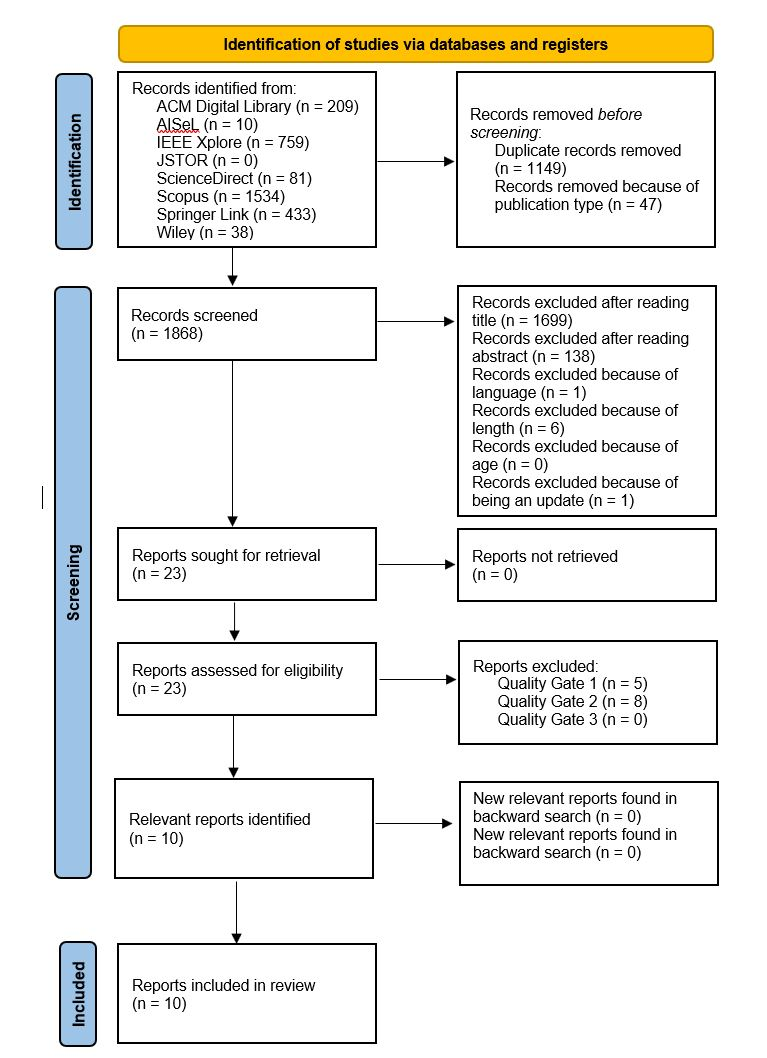
\includegraphics[width=8cm]{Media/PRISMA-Flowchart-V2.JPG}
    \caption{Overview of the search process}
    \label{fig:PRISMA}
\end{figure}

\subsubsection{Evaluating papers based on inclusion and exclusion criteria}

In the initial phase, 1,196 papers have been removed due to duplication and publication type. The remaining 1868 papers were filtered by title to evaluate their relevance to the concepts of microservice patterns or architectural constructs related to MS. For this purpose, the first two authors separately evaluated each entry. If both agreed, this verdict was honored. In case of disagreement, they discussed the title to come to a conclusion. In this phase, the first author initially included 113 papers and the second author 146. Of those, 41 were present in both sets and 1650 were excluded by both. This equates to an agreement rate of 90,5 percent (1691 of 1868 records) between the authors. After discussing the contributions with divergent evaluations, in total, 1699 of the 1868 papers were excluded, leaving 169 items for the next round. 

The same approach was followed for abstracts. As a result, the first author evaluated 40 papers positively, and the second one 28. Both agreed on the exclusion of 138. From there on, the papers that were not written in English (despite the abstract being in English), were published before the year 2012, and had a length of less than six pages were removed. 23 papers have been selected for the quality assement against the quality framework. The agreement rate among researchers for this phase equates to 88 percent. 

% It was stipulated so if the agreement could not be reached, an arbitrator would be invited to the research Yet, this was not necessary. 



% With a difference that authors agreed to also allow themselves to look into the actual paper and not just the abstract, if they wanted to further explore certain aspects of the study to improve their judgement.



% While conducting the first steps of our filter process, we encountered several hurdles that shall be highlighted to ensure transparency, especially since they can slightly affect the number of remaining entries after those initial phases. However, the final set of literature was not impacted and, therefore, those factors did not pose a threat to the studies validity. For once, since not all entries of the combined literature list specified a digital object identifier (DOI), the duplicate removal had to be conducted based on the publication title. Yet, in some rare cases, there were duplicates for which the spelling of the title was slightly altered (e.g., the two parts of a title were in one search engine separated by a hyphen and in another by a double colon), and which were, therefore, not detected in the initial duplicate removal phase. Instead, they were only identified during the scanning of the title. 

% Furthermore, in SpringerLink, conference papers are classified as book chapter, since conference proceedings are published as books. This makes them indistinguishable from real book chapters, when only looking at the metadata. Book chapters are, however, not part of the search’s scope. Consequently, the removal of book chapters for SpringerLink could only be processed when inspecting the respective publications. To slightly reduce the effort, it was decided to only do this for those publications that passed the filtering by title.


% However, while there were three corresponding records in the initially obtained set of literature (from the years 2003, 2007, and 2010), those were already filtered out for other reasons by this stage. 


\subsubsection{Evaluating papers based on the quality framework}

After having filtered out the pooled studies based on inclusion and exclusion criteria, we initiated a deeper probing, by running the remaining studies against the quality framework. The filtering based on the quality criteria was divided into three differently focused phases, with each of them requiring the passing of a quality gate as portrayed in Table \ref{qualityFramework}. In the first phase, the aim was to ensure that reports fulfill at least a desired minimum level of comprehensiveness. For this purpose, studies were evaluated for their content to see if they are actual research or just a mere report on some lessons or expert opinions. In addition, we checked if objectives, justification, aim and context of the studies are clearly communicated.

% This last criterion is primarily geared towards actual experiments. In the conducted literature search, primarily literature-based studies were found, which somewhat devalues this aspect. Nevertheless, to assure completeness, it was still evaluated. 


Authors independently rated the three aspects for all 23 remaining papers, giving one point respectively, if they deemed a criterion fulfilled and no point if they considered that aspect lacking. Consequently, for each aspect, zero to two points were achievable and for all aspects, six points were available per paper. For inclusion into the second phase, at least five out of six points were demanded to assure a sufficient base quality. This corresponds to having at least 75 percent of the points. 

% Two papers that obtained four out of six points were again discussed between the two authors to avoid any erroneous exclusion.

% Despite that additional check, both were still removed. 

In total, the authors agreed on 51 of 69 evaluations, resulting in an agreement rate of 73,9 percent. The second phase was focused on rigor. In this phase, studies were judged based on their research design and the data collection methods. The general procedure with the first two authors independently evaluating the reports remained the same. For inclusion in the next phase, again, 75 percent of the obtainable point were needed (this time three out of four). In total, the authors agreed on 23 of 36 evaluations, resulting in an agreement rate of 63,9 percent. While this value is rather low, this is likely caused by the narrow margins for some decisions. 

Once more, the papers with the highest score (this time two) were discussed before inclusion, to further counteract possible fuzziness in the individual evaluations.  The remaining 10 papers went through the third and final phase. Here, the credibility of the reporting and the relevance of the findings were evaluated. The procedure was the same as the previous phases. However, this time, all of the remaining papers passed. In this last phase, the authors agreed on 14 of 20 evaluations, resulting in an agreement rate of exactly 70 percent. 






% TBC
% The final set of literature that is the output of the conducted review process is shown in Table 4.  




\subsubsection{Forward/backward Search}

To further increase the comprehensiveness of the review process, following the recommendation of Webster and Watson \cite{webster2002analyzing}, the initial keyword search was amended with a forward and backward search. Here, for the identified ten papers it was examined by which papers they are cited and which papers they cite. This was performed between October 10, 2022 and October 20, 2022. While the backward search could simply be based on the reference lists given in the papers, the forward search was less unequivocal, because there are several sources with slightly varying information. To account for this, two different ones, namely Google Scholar and ResearchGate were used. 

However, both searches yielded no new results that sufficed the criteria applied in the initial search. 
Instead, the 538 papers (combined for all papers and both sources, not accounting for duplicates) found in the forward search comprised, inter alia, thesis works, preprints, studies that are not directly related to microservices, papers that are too short and papers that did not meet the quality criteria. Regarding the backward search, most of the utilized conference papers and journal articles with a focus on microservices were already captured by the initial search, further highlighting its comprehensiveness. In total for the ten papers, and not accounting for duplicates, there were 16 new entries mentioning microservices in the title that were, however, ultimately not relevant for the focus of this work. Therefore, the final set still consists of the ten contributions shown in Table~\ref{finalLiterature}.

\begin{table}[!ht]
  \renewcommand{\arraystretch}{1.5}
  \caption[]{The final set of literature}
  \begin{tabular}{|p{0.3cm}|p{4cm}|p{0.7cm}|p{0.8cm}|p{0.5cm}|p{2cm}|p{1cm}|p{0.5cm}|}
      \hline
      ID & Title & Year & Quality Score & Type & Source & Found in & Ref  \\ 

      \hline

      S1 & Architectural patterns for microservices: A systematic mapping study & 2018 & 11/14 & C & CLOSER 2018 - Proceedings of the 8th International Conference on Cloud Computing and Services Science & Scopus & \cite{Taibi.2018} \\ 
      \hline
      S2 & Actual Use of Architectural Patterns in Microservices-Based Open Source Projects & 2018 & 12/14 & C & Proceedings of the 25th Asia-Pacific Software Engineering Conference (APSEC) & Scopus, IEEE Xplore & \cite{Marquez.2018}  \\ 
      \hline  
      S3 & Supporting architectural decision making on data management in microservice architectures & 2019 & 12/14 & C & Lecture Notes in Computer Science 11681
      Proceedings of the Software Architecture: 13th European Conference, ECSA 2019 & Scopus, SpringerLink & \cite{Ntentos.2019}  \\ 

      \hline  
      S4 & Using architectural modifiability tactics to examine evolution qualities of Service- and Microservice-Based Systems: An approach based on principles and patterns & 2019 & 13/14 & J & Software-Intensive Cyber-Physical Systems & Scopus & \cite{Bogner.2019} \\ 
      \hline   
      S5 & Patterns Related to Microservice Architecture: a Multivocal Literature Review & 2020 & 14/14 & J & Programming and Computer Software & Scopus, SpringerLink & \cite{Valdivia.2020}  \\ 
      \hline
      S6 & Data management in microservices: State of the practice, challenges, and research directions & 2021 & 12/14 & J & Proceedings of the VLDB Endowment 2021 & Scopus & \cite{Laigner.2021}  \\ 
      \hline
      S7 & Deployment and communication patterns in microservice architectures: A systematic literature review & 2021 & 14/14 & J & Journal of Systems and Software & Scopus, ScienceDirect & \cite{aksakalli2021deployment}  \\ 
      \hline
      S8 & Decision Models for Selecting Patterns and Strategies in Microservices Systems and their Evaluation by Practitioners & 2022 & 13/14 & C & Proceedings of the 2022 IEEE/ACM 44th International Conference on Software Engineering: Software Engineering in Practice (ICSE-SEIP) & IEEE Xplore & \cite{Waseem.2022} \\ 
      \hline
      S9 & Designing Microservice Systems Using Patterns: An Empirical Study on Quality Trade-Offs & 2022 & 13/14 & C & IEEE 19th International Conference on Software Architecture (ICSA) & IEEE Xplore & \cite{Vale.2022} \\ 
      \hline
      S10 & Taxonomical Classification and Systematic Review on Microservices & 2022 & 13/14 & J & International Journal of Engineering Trends and Technology & Scopus & \cite{Weerasinghe.2022}  \\ 
      \hline
  \end{tabular}
  \label{finalLiterature}
\end{table}

All ten publications have been published in 2018 or later, with three of them being published in 2022, which shows the timeliness of the topic. Eight of the ten papers were found via Scopus, whereas the remaining two have been identified through IEEE Xplore. 




\subsubsection{The found papers}

To give an overview of the papers found in the literature review and, thereby, also provide context to the extracted knowledge, they are briefly described in the following:

\begin{description}
  \item[S1:] In \cite{Taibi.2018}, the authors conducted a systematic mapping study to identify microservice architecture patterns, create a corresponding catalogue that gives an overview of advantages and disadvantages, and, thereby, provide support developers in finding suitable solutions for their own needs. The initial search for literature yielded 2754 unique papers that were filtered for suitability, resulting in a final set of 42 contributions from conferences, workshops, journals, and grey literature. Besides describing the patterns and outlining in which papers their use has been described, the authors also highlighted the guiding principles of the microservice approach in general. Further, corresponding trends and open issues are discussed, amending the given comprehensive overview.
  \item[S2:] The use of architectural patterns in open source projects that are based on microservices is addressed in \cite{Marquez.2018}. Similar to the previous one, this article also presents a catalog of microservices architectural patterns based on literature. Further, it relates them to quality attributes, compares them to patterns that are found in service oriented architectures, and investigates which patterns are used in microservice-based open source projects. While the general review process seems reasonable, it lacks a reporting of the number of papers assessed in each stage. However, including repeated mentioning across papers, the final set of 16 papers yielded 164 architectural patterns, with 52 stemming from academic papers and 112 from industrial ones. After further processing, those were reduced to 17 patterns that were deemed the most relevant and discussed in more detail.
  \item[S3:] A review that is focused on the data management in the context of microservices is presented in \cite{Ntentos.2019}. For this purpose, instead of exploring the scientific body of literature, the grey literature was targeted, since much of the corresponding knowledge can be found in experience reports, blog entries, or system documentations, which makes it hard to obtain a comprehensive overview. In total, 35 contributions from practitioners were qualitatively explored, analysing, which patterns and practices were used by them, and which factors influenced their architectural decisions. Based on the findings, a model was proposed that formalizes the corresponding decisions and thereby facilitates a more comprehensive understanding of the domain.
  \item[S4:] The modifiability of software and how it is influenced by the service-oriented architecture (SOA) as well as microservices is examined in \cite{Bogner.2019}. For this purpose, the authors firstly compiled a list of fifteen architectural modifiability tactics and mapped those with eight service-oriented design principles and eight microservice principles they extracted from selected publications. Subsequently, they presented the results of the mapping and discussed the results. Further, they analysed the relations of 42 microservice and 118 SOA patterns with the modifiability tactics. As with the principles, the patterns were also obtained by consulting specific selected publications. The identified relations are presented and the overall findings discussed, providing the reader with a rather comprehensive insight in the interplay of architectural modifiability, microservices, and SOA.
  \item[S5:] A review on the relationship between microservice patterns, quality attributes, and metrics is given in \cite{Valdivia.2020}, which is an updated and extended version of the authors' previous work. To provide a comprehensive overview, both, scientific literature and grey literature were considered. While initially 605 results were found through the keyword search, the filtering reduced that number to 18. By backward snowballing for the grey literature, this number was increased to 27 for the final set that comprises 13 scientific papers and 14 from grey literature. In total, 54 patterns were identified. However, some of them are strongly related to each other or even redundant. The authors could link the identified patterns to six quality characteristics. Further, they assigned the patterns to one of six groups based on the provided benefits and analysed how many papers from scientific literature and grey literature are related to each group. Moreover, they also provided a comprehensive qualitative discussion of the groups, the respective patterns and the development over time.
  \item[S6:] A second literature review on data management in a microservice context is presented in \cite{Laigner.2021}. For this purpose, a systematic literature review was conducted, where 300 peer-reviewed papers were analysed, leading to a final selection of 10 articles the authors deemed representative. Further, 9 microservice-based applications were analysed that were chosen from `more than 20' \cite{Laigner.2021} open-source project. Additionally, an online survey with more than 120 participants was conducted. In doing so, the authors found out that state-of-the-art database systems are often insufficient for the needs of practitioners, which leads to them combining multiple heterogeneous systems to fulfil their tasks. This, in turn, reduces the importance of database systems when dealing with microservices, since they often only provide data storage functionalities, with the data management logic being shifted to the application layer. Moreover, the data management logic and the common types of queries as well as the major challenges regarding the data management are discussed. Finally, the requirements for database management systems in the context of microservices are highlighted and avenues for future research are outlined.
  \item[S7:] Microservice related deployment and communication patterns were collected in \cite{aksakalli2021deployment}. This was done by conducting a systematic literature review, in which initially 440 items were reviewed, with 34 primary studies being selected as relevant and amended by 4 additional contributions that were found by backward and forward snowballing. Subsequently, the final set is comprehensively presented regarding multiple quality metrics and the applied research methods. In the analysis part, the authors extensively discuss the varying deployment approaches and communication patterns for microservices. Further, they highlight the corresponding obstacles and issues, and promising directions for future research. The work is concluded by a comprehensive overview of its key findings, which are also visualized in the form of a taxonomy. 
  \item[S8:] The selection of patterns and strategies in microservice systems is targeted in \cite{Waseem.2022}. For this purpose, the authors developed and evaluated four decision models that use requirements, in this case desired quality attributes, as input and output appropriate design elements. The models are also the main contribution of this work. Each of the models is focused on one specific theme. These are application decomposition, security, communication, and service discovery. As a foundation for the creation of the models, they searched the existing scientific and grey literature. From an initial set of 2110 publications, they kept 39 scientific papers and 23 grey literature items. Those contained 211 patterns and strategies for the former and 174 for the latter. After duplicate removal, there were 7 patterns and strategies left for application decomposition into microservices, 8 related to security, 15 for microservices communication, and 6 for service discovery. Each of them is briefly summarized and the advantages and disadvantages with respect to the quality attributes is discussed.
  \item[S9:] How the use of patterns for the development of microservice systems affects the quality is examined in \cite{Vale.2022}. Further, it is regarded, how and why patterns are adopted in microservice systems and how quality attributes in a microservice context can be measured. However, at first, the authors introduce and describe the seven quality attributes that are used as foundation for the work. To gather new insights, the authors conducted nine semi-structured face-to-face interviews with practitioners and and microservice experts. They were questioned regarding the use of the 14 patterns from the “design and implementation” category of the cloud design patterns catalogue \cite{AAC.2022} provided in the Azure Architecture Center by Microsoft. These are described, the degree of use by the interviewees is stated, and they are linked with the quality attributes. Further, the advantages and disadvantages stated by the interviewees are compared with those that were already present in the documentation of the patterns catalogue.
  \item[S10:] The list is concluded by a paper that focusses on a rather broad overview of the microservice domain \cite{Weerasinghe.2022}. For this purpose, a systematic literature review, following the PRISMA model \cite{Page.2021} was conducted. Hereby, an initial collection of 4056 items was reduced to a final set of 49 papers. The primarily regarded topics are the motivators for the conversion from a monolithic architecture to a microservice architecture, which technologies and architectural patterns occur in modern systems and which challenges arise when using the microservice architecture. Additionally, future trends are discussed. Here, the the increasing importance of cloud computing is highlighted. Other themes are the need to assure a low latency, due to the inherent inter-service communication, as well as the required skill for the development, which could be somewhat counteracted by the development of corresponding tools.
\end{description}

























\subsubsection{Data synthesis}

After selecting the quality papers, we embarked on the data synthesis process. For this phase we follow the guidelines of thematic synthesis discussed by Cruzes et al. \cite{Cruzes.2011}. To begin, we first extracted the following data from each paper: 1) findings, 2) research motivation, 3) author, 4) title, 5) research objectives, 6) research method, 7) year. We extracted these data through coding, using the software Nvivo. After that, we created two codes: 1) patterns, and 2) quality attributes, and coded the findings based on it. By the end of this process, various themes emerged.



 



\subsection{Second Review} \label{secondReview}

The second SLR is conducted by \cite{ataei2022state} on available BD RAs in academia and industry. This is comprehensive study that covers various aspects of BD RAs such as limitations, and common architectural blocks. The findings from this SLR helped us shaped the requirements necessary for BD systems. We do not explore this SLR in this paper, and aim to only discuss the results of it.

% The second SLR was the less extensive one, since it is just an update to an already existing study. For this purpose, the SLR conducted by Ataei et al. \cite{Ataei.2020}, was extended up unto the current date, providing us with the necessary overview. The original study covered up to 2020, ths we followed the same methodology as discussed in Section~\ref{firstReview} with the following difference: 

% \begin{enumerate}
%   \item inclusion criteria for this SLR covers the years 1st 2010 and 10th October 2022 
%   \item inclusion criteria for this SLR selects studies that are focused on BD architecture, BD reference architectures, and BD system and software requirements.
%   \item our Nvivo codes are as following: 1) BD Architectural components, 2) BD requirements, 3) Fundamental concepts of BD RAs
%   \item the keywords searched are illustrated in Table \ref{searchTermsSecond}
% \end{enumerate}

% \begin{table*}
%   \renewcommand{\arraystretch}{1.5}
%   \caption[]{Mapping of databases/registers and search terms for the second review}
%   \begin{tabular}{|p{2.8cm}|p{7cm}|p{1.5cm}|}
%       \hline
%       Database/Register & Search Term & Records \\ 

%       \hline
%       ACM Digital Library (“The ACM Full-Text Collection”, not “The ACM Guide to Computing Literature
%       &  
      
%       [Title: big data] AND [[Title: reference architecture*] OR [Title: big data architecture]

%       & 
%       696
      
%       \\ 

%       \hline
%       AISeL & \textbf{Title}: microservice OR microservices & 11 \\ 
%       \hline

%       IEEE Xplore & ("Document Title":big data) AND ("Document Title":reference architecture) OR ("Document Title":big data ) AND ("Document Title":architecture)
      
%       & 302  \\ 
%       \hline

%       JSTOR & 
      
%       \textbf{Title:} 1) big data reference architecture 

%       \textbf{Title:} 2) big data architecture 
%       & 
      
%       1) 6,682


%       2) 671

%       \\ 

%       \hline

%       ScienceDirect & 
      
%     \textbf{Title}: big data AND ( reference architecture OR architecture )

%       & 
%        70 

%       \\ 

%       \hline

%       Scopus &

%       ( TITLE ( big  AND  data  AND  reference  AND  architecture )  OR  TITLE ( big  AND data  AND architecture ) ) 
      
%       & 
      
%       814 
      
%       \\ 
%       \hline

%       SpringerLink & \textbf{Title}: big data


%       \textbf{With at least one of the words}: architecture reference architecture

%        & 27 \\ 
%       \hline

%       Wiley & 
%       \textbf{Title}: 1) big data reference architecture  
      
%       \textbf{Title}: 2) big data architecture
%       & 
%       1) 1


%       2) 132
      
%       \\ 

%       \hline
%   \end{tabular}
  
%   \label{searchTermsSecond}
% \end{table*}

% In the first phase of this SLR, a total of 138 literature has been pooled from academia, and 24 from grey literature. Some of this literature has been added to the pool by the process of forward and backward searching. For instance, by reading NIST RA \cite{Chang.2019}, we found out about Oracle, Facebook, and Amazon RAs and included those in the pool of the literature as well. 

% In the screening phase, the literature that were not in-line with our inclusion and exclusion criteria have been eliminated. For example, if the paper was very short and was not on the topic of BD RA, or its ecosystem or limitations, it was excluded. As a result of this phase, 50 papers excluded. In the next phase, by assessing studies against the quality framework, 21 studies from academia, and 12 studies from grey literature pool has been eliminated.

% Finally, 79 studies have been selected comprising of proceedings, journal articles, book chapters, and white papers. Out of the pool of articles, 33.3\% are from IEEE Explore, 5.2\% from ScienceDirect, 24.5\% from SpringerLink, 15.7\% from ACM, and 21\% from other sources such as Google Scholar, Research Gate and gray literature. 30 journal articles, 29 conference proceedings, 12 book chapters, 6 white papers, 1 Master’s Thesis and 1 PhD thesis were selected. 55\% of the articles were selected from the years 2016- 2022, 33\% belonged to years 2013-2016, and the rest to years 2010-2013. The PRISMA flowchart is depicted in Figure~\ref{fig:PRISMA}.

% \begin{figure*}[t]
%   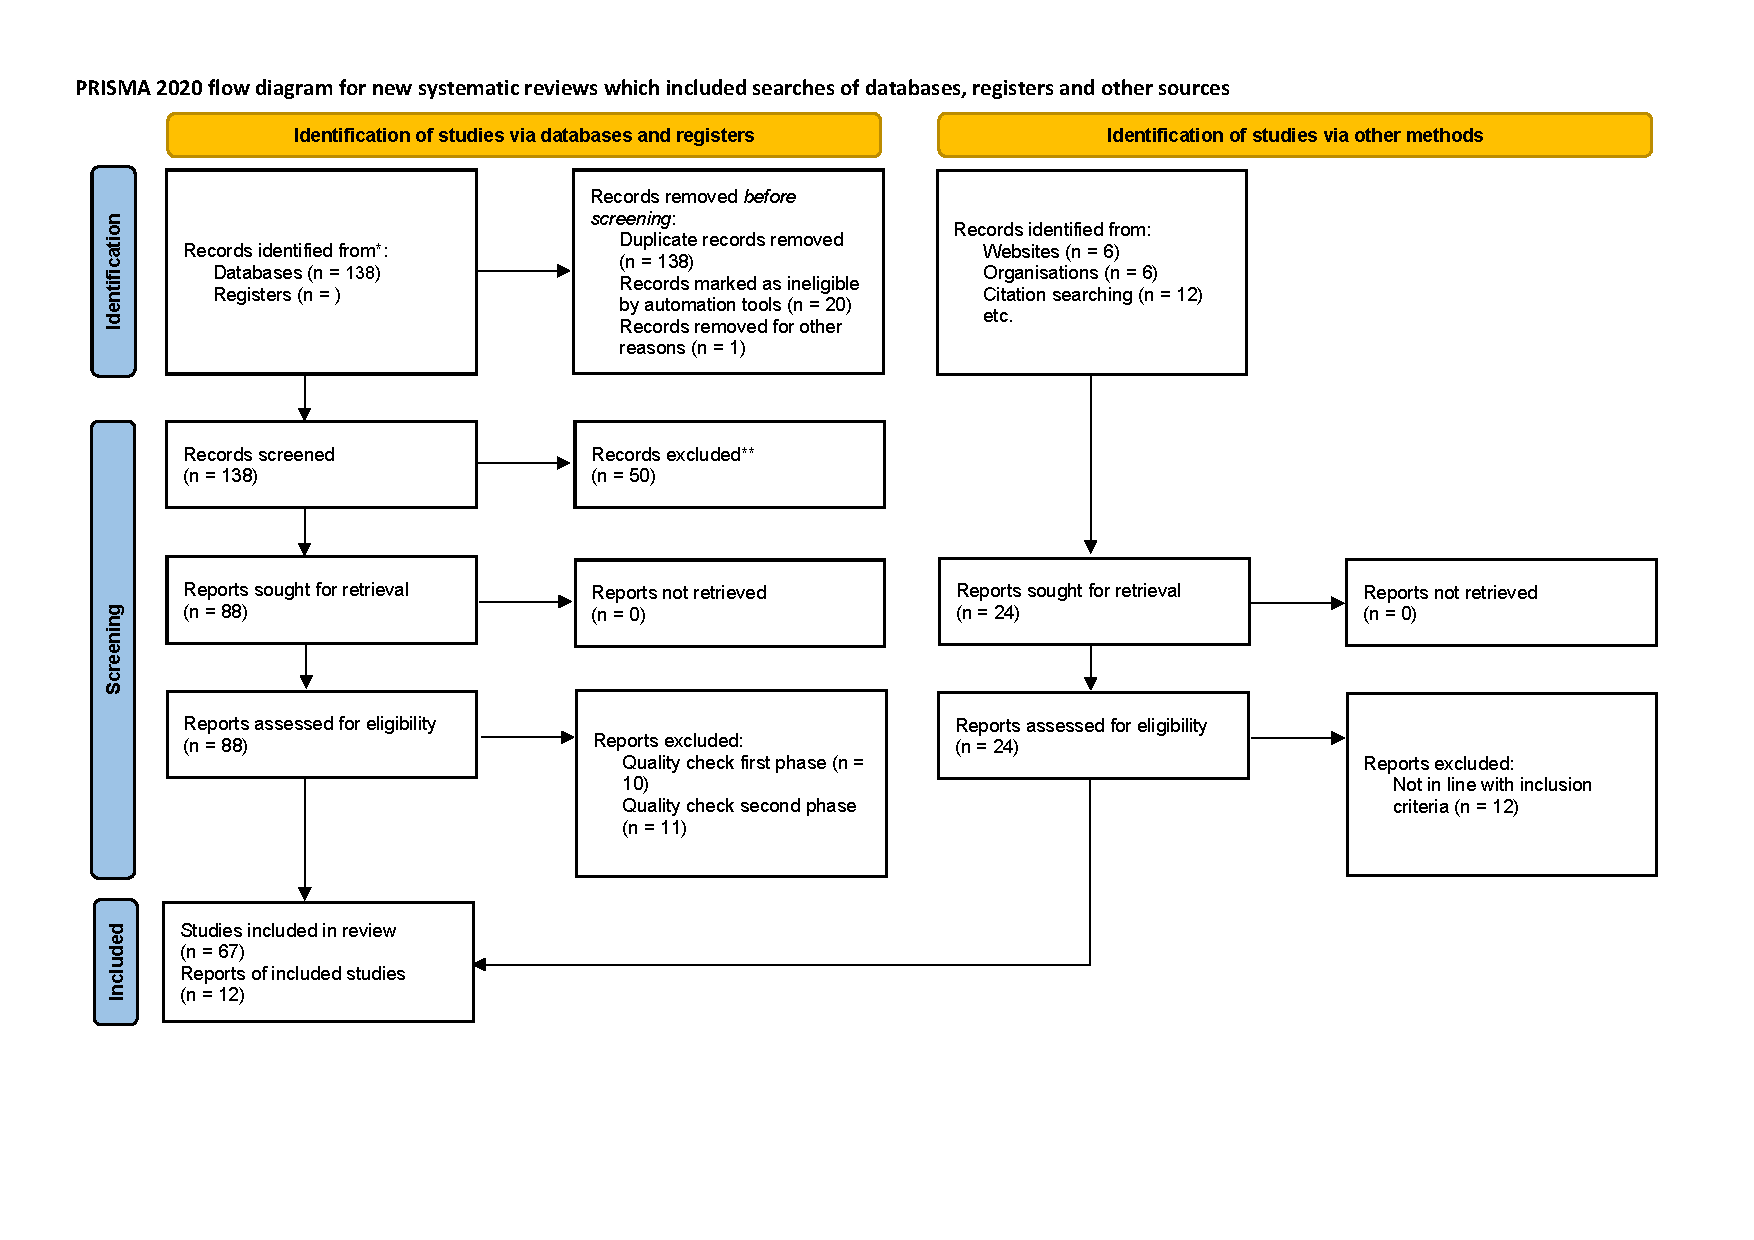
\includegraphics[width=13cm]{PRISMA/PRISMA_Flow_Diagram-2.pdf}
%   \caption{PRISMA flowchart}
%   \label{fig:PRISMA}
% \end{figure*}

% By the result of this SLR, 22 BD RAs have been found as portrayed in Table \ref{table:bdRAs}. By analyzing these RAs and the theory that derives them, two kinds of theory have been attained: 1) software and system requirements  as per the Section~\ref{requirementSpec} 2) design theories and architectural constructs as per the Section~\ref{Mapping}.


% \begin{table*}
%   \renewcommand*{\arraystretch}{1.4}
%   \caption{BD RAs}
%   \label{table:bdRAs}
%   \begin{tabular}{|p{0.4cm}|p{9cm}|p{1.2cm}|p{0.5cm}|}
%   \hline
%   \textbf{ID} & \textbf{Title} & \textbf{Domain} & \textbf{Year} \\
%   \hline
%   s1 & Lambda architecture (\cite{kiran2015lambda} ) & Practice  &  2011   \\
%   \hline
%   s2 & IBM - Reference architecture for high performance analytics in healthcare and life science (\cite{quintero2019ibm} ) & Practice  &  2013   \\
%   \hline
%   s3 &  Microsoft - Big Data ecosystem reference architecture  (\cite{levin2013big} ) & Practice  &  2013   \\
%   \hline
%   s4 &  Oracle - Information Management and Big Data: A Reference Architecture  (\cite{cackett2013information} ) & Practice  &  2014   \\
%   \hline
%   s5 & Towards a big Data reference architecture (\cite{Maier} ) & Academia  &  2013   \\
%   \hline
%   s6 & A reference architecture for Big Data solutions introducing a model to perform predictive analytics using Big Data technology (\cite{geerdink2013reference} ) & Academia  &  2013   \\
%   \hline
%   s7 & A proposal for a reference architecture for long-term archiving, preservation, and retrieval of Big Data (\cite{viana2014proposal} ) & Academia  &  2014   \\
%   \hline
%   s8 & Questioning the Lambda architecture; Kappa Architecture (\cite{kreps2014questioning} ) & Academia  &  2014   \\
%   \hline
%   s9 & Accelerating Secondary Genome Analysis Using Intel Big Data Reference Architecture. (\cite{SikoraWohlfeld2014} ) & Practice  &  2014  \\
%   \hline
%   s10 & Reference architecture and classification of technologies, products and services for big data systems (\cite{paakkonen2015reference} ) & Academia  &  2015   \\
%   \hline
%   s11 &  SAP - NEC Reference Architecture for SAP HANA \& Hadoop (\cite{SAPRA} ) & Practice  &  2016   \\
%   \hline
%   s12 & Big data architecture for construction waste analytics (CWA ): A conceptual framework (\cite{bilal2016big} ) & Academia  &  2016   \\
%   \hline
%   s13 & A reference architecture for Big Data systems in the national security domain (\cite{Klein} ) & Academia  &  2016   \\
%   \hline
%   s14 & Managing Cloud-Based Big Data Platforms: A Reference Architecture and Cost Perspective (\cite{heilig2017managing} ) & Academia  &  2017   \\
%   \hline
%   s15 & A software reference architecture for semantic-aware Big Data systems; Bolster Architecture (\cite{Nadal} ) & Academia  &  2017   \\
%   \hline
%   s16 & Simplifying big data analytics systems with a reference architecture (\cite{sang2017simplifying} ) & Academia  &  2017   \\
%   \hline
%   s17 & NIST Big Data interoperability framework (\cite{Chang} ) & Practice  &  2018  \\
%   \hline
%   s18 & Extending reference architecture of big data systems towards machine learning in edge computing environments (\cite{paakkonen2020extending} )  & Academia & 2020   \\
%   \hline
%   s19 & A Big Data Reference Architecture for Emergency Management (\cite{iglesias2020big} )  & Academia & 2020   \\
%   \hline
%   s20 & ISO/IEC 20547-3:2020 BS ISO/IEC 20547 3:2020 Information technology. Big data reference architecture. Reference architecture (\cite{ISO20547} ) & Practice  &  2020  \\
%   \hline
%   s21 & Phi: A Generic Microservices-Based Big Data Architecture (\cite{maamouri2021phi} )  & Academia & 2021   \\
%   \hline
%   s22 & NeoMycelia: A software reference architecturefor big data systems (\cite{AtaeiApsec} )  & Academia & 2021   \\
%   \hline
%   \end{tabular}
% \end{table*}

% Consequently, for the search conducted for this paper, the other databases and registers have not been necessary. However, since this fact is only determinable now, their inclusion in the initial search was still sensible.

% % Pouya


\section{Results}

In this section, we present with three integral elements: 1) BD requirements, 2) MS patterns, 3) the mapping between the two and theories that emerged as a result.  

\subsection{Requirements specification} \label{requirementSpec}

The results of our data synthesis emerged a few themes in regards to BD requirements. While we could find BD major building blocks and system requirements from the result of our SLR, our SLR did not include categorization and representation of these requirements. We also did not know what type of requirements is the most suitable to the goal of this study. To this end, we performed a lightweight literature review in the body of knowledge to realize three major elements: 1) the type of requirements that we need, 2) an approach to categorizing the requirements, 3) presentation of these requirements. 

\subsubsection{Type of requirements}
System and software requirements come in different flavours and can range from a formal (mathematical) specifications to sketch on a napkin. There's been various attempts to defining and classifying software and system requirements. For the purposes of this study, we opted for a well-received approach discussed by Laplante \cite{laplante2017requirements}. In this approach, requirements are classified into three major types of 1) functional requirements, 2) non-functional requirements, and 3) domain requirements. 

Our objective is to define the high-level requirements of BD systems, thus we do not fully explore 'non-functional' requirements. Majority of non-functional requirements are emerged from the particularities of an environment, such as a banking sector or healthcare, and do not correlate to our study. Our primary focus is one functional and domain requirements. 

\subsubsection{Categorizing requirements} After having filtered out the right type of requirement, we then sought for a rigorous and relevant method to categorize the requirements. For this purpose, we followed the well-established categorization method based on BD characteristics, that is the 5Vs. These 5Vs are velocity, veracity, volume, Variety and Value \cite{Bughin2016}, \cite{rad2017big}. We took inspiration from various studies such as Nadal et al. \cite{nadal2017software}, and the requirements categories presented in NIST BD Public Working Group \cite{Chang.2019}.

% have underpinned their reference architecture on these characteristics and requirements that goes with them. Moreover, NIST BD Public Working Group embarked on a large scale study to extract requirements from variety of application domains such as Healthcare, Life Sciences, Commercial, Energy, Government, and Defense. The result of this study was the formation of general requirements under seven categories. In another effort by Volk et al. (\cite{volk2020identifying}), nine use cases for BD projects are identified by collecting theories and use cases from the literature and categorizing them using a hierarchical clustering algorithm. 

% Bashari et al. (\cite{bashari2016security}) focused on the security and privacy requirements of BD systems, Yu et al. presented the modern components of BD systems (\cite{yu2019components}), Eridaputra et al. (\cite{eridaputra2014modeling}) created a generic model for BD requirements using goal oriented approaches, and Al-jaroodi et al. (\cite{al2016characteristics}) investigated general requirements to support BD software development. 

We've also studied the reference architectures developed for BD systems to understand general requirements. The result of the second SLR presented 22 RAs from academia and industry. This study helped us realize the spectrum of BD reference architectures, how they are designed and the general set of requirements. By analyzing these studies and by evaluating the design and requirement engineering required for BD reference architectures, we adjusted our initial categories of requirements and added security and privacy to it. 

\subsubsection{Present requirements}
After knowing the type and category of requirements, We looked for a rigorous approach to present these requirements. There are numerous approaches used for software and system requirement representation including informal, semiformal and formal methods. For the purposes of this study, we opted for an informal method because it is a well established method in the industry and academia \cite{kassab2014state}. Our approach follows the guidelines explained in ISO/IEC/IEEE standard 29148 \cite{ISO29148} for representing functional requirements. We have also taken inspiration from Software Engineering Body of Knowledge \cite{abran2004software}. However, our requirement representation is organized in term of BD characteristics. These requirements are described in following sub-sections.

% Table \ref{table-requirements}. 

% \begin{table*}[h]
%     \centering
%     \caption{BD system requirements}
%     \renewcommand*{\arraystretch}{1.8}
%     \begin{tabular}{|m{1.2cm}|m{10.5cm}|}

%         \hline

%         Volume &

%         \textbf{Vol-1)} System needs to support asynchronous, streaming, and batch processing to collect data from centralized, distributed, and other sources, \textbf{Vol-2)} System needs to provide a scalable storage for massive data sets 
%         \\
%         \hline
%         Velocity & 
        
%         \textbf{Vel-1)} System needs to support slow, bursty, and high-throughput data transmission between data sources, \textbf{Vel-2)} System needs to stream data to data consumers in a timely manner, \textbf{Vel-3)} System needs to be able to ingest multiple, continuous, time varying data streams, \textbf{Vel-4)} System shall support fast search from streaming and processed data with high accuracy and relevancy, \textbf{Vel-5)} System should be able to process data in real-time or near real-time manner 
%         \\ 

%         \hline

%         Variety & 

%         \textbf{Var-1)} System needs to support data in various formats ranging from structured to semi-structured and unstructured data, \textbf{Var-2)} System needs to support aggregation, standardization, and normalization of data from disparate sources, \textbf{Var-3)} System shall support adaptations mechanisms for schema evolution, \textbf{Var-4)} System can provide mechanisms to automatically include new data sources 
%         \\

%         \hline

%         Value & 
        
%         \textbf{Val-1)} System needs to able to handle compute-intensive analytical processing and machine learning techniques, \textbf{Val-2)} System needs to support two types of analytical processing: batch and streaming, \textbf{Val-3)} System needs to support different output file formats for different purposes, \textbf{Val-4)} System needs to support streaming results to the consumers 
%         \\

%         \hline

%         Security \& Privacy & 
        
%         \textbf{SaP-1)} System needs to protect and retain privacy and security of sensitive data, \textbf{SaP-2)} System needs to have access control, and multi-level, policy-driven authentication on protected data and processing nodes. 
%         \\

%         \hline
        
%         Veracity &
        
%         \textbf{Ver-1)} System needs to support data quality curation including classification, pre-processing, format, reduction, and  transformation, \textbf{Ver-2)} System needs to support data provenance including data life cycle management and long-term preservation.
%         \\
%         \hline
  
%     \end{tabular}
%     \label{table-requirements}
%     \end{table*}


\setlist{leftmargin=1.5cm,before=\vspace{\baselineskip}}

\paragraph{Volume}

Volume refers to addressing multitude of data for the purposes of storage and analysis. An architecture needs to be elastic enough to address volume demands at different rates. Storing and computing large volume of data with attention to efficiency is a complex process that requires distributed and parallel processing. Therefore, volume requirements are as following:
`'
% in Table \ref{table-requirements}. These requirements are mapped against our components discussed in \ref{the-artifact}.

\begin{enumerate}[label=\textbf{Vol-\arabic*}]
    \item System needs to support asynchronous, streaming, and batch processing to collect data from centralized, distributed, and other sources
    \item System needs to provide a scalable storage for massive data sets
\end{enumerate}


\paragraph{Velocity}

Velocity refers to addressing the rate at which data flows into system for different analytical requirements. Processing of data to expedite the decision-making process quickly on one hand and handling the variety of data and storing them for batch processing, stream processing or micro-batch processing on other hand bring considerable technical challenge. Therefore, velocity requirements are as following: 

\begin{enumerate}[label=\textbf{Vel-\arabic*}]
    \item System needs to support slow, bursty, and high-throughput data transmission between data sources
    \item System needs to stream data to data consumers in a timely manner
    \item System needs to be able to ingest multiple, continuous, time varying data streams
    \item System shall support fast search from streaming and processed data with high accuracy and relevancy
    \item System should be able to process data in real-time or near real-time manner
\end{enumerate}


\paragraph{Variety}

Variety refers to addressing data in different format, such as structured, unstructured, and semi-structured. Different formats may require different processing techniques, may have different storage requirements and may be optimized in different ways. Hence, an effective BD architecture can handle various data types and enable the processing and transformation of them in an efficient manner. Therefore, the variety requirements are as following: 

\begin{enumerate}[label=\textbf{Var-\arabic*}]
    \item System needs to support data in various formats ranging from structured to semi-structured and unstructured data
    \item System needs to support aggregation, standardization, and normalization of data from disparate sources,
    \item System shall support adaptations mechanisms for schema evolution
    \item System can provide mechanisms to automatically include new data sources
\end{enumerate}


\paragraph{Value}

Value refers to addressing the process of knowledge extraction from large datasets. Value is perhaps one of the most challenging aspects of BD architecture as it involves a variety of cross-cutting concerns such as data quality, metadata and data interoperability. Gleaning, crunching and extracting value from data, requires an integrated approach of storage and computing. Value requirements are as following:

\begin{enumerate}[label=\textbf{Val-\arabic*}]
    \item System needs to able to handle compute-intensive analytical processing and machine learning techniques
    \item System needs to support two types of analytical processing: batch and streaming
    \item System needs to support different output file formats for different purposes
    \item System needs to support streaming results to the consumers 
\end{enumerate}

\paragraph{Security and Privacy}

Security and privacy should be some of the top concerns for the design of any effective BD system. An effective architecture should be secure, adopting the best security practices (principles of least privilege) and in the meantime respect regional and global privacy rules (GDPR for example). The security and privacy requirements are as following:

\begin{enumerate}[label=\textbf{SaP-\arabic*}]
    \item System needs to protect and retain privacy and security of sensitive data
    \item System needs to have access control, and multi-level, policy-driven authentication on protected data and processing nodes.
\end{enumerate}

\paragraph{Veracity}

Veracity refers to keeping a certain level of quality for data. Data veracity refers to truthfulness and accuracy of data; in simpler terms, it is to ensure that data possess qualities necessary for crunching and analysis. Veracity requirements are as following: 

\begin{enumerate}[label=\textbf{Ver-\arabic*}]
    \item System needs to support data quality curation including classification, pre-processing, format, reduction, and transformation
    \item System needs to support data provenance including data life cycle management and long-term preservation
\end{enumerate}



\subsection{Microservice Patterns}



As a result of this SLR, our data synthesis yielded 28 MS patterns. These patterns are classified based on their function and the problem they solve. Our categories are inspired by the works of Richardson \cite{Richardson.2022}. These categories can be seen in Table \ref{microservices-categorization}. While we elaborate the patterns adopted for BD requirements in detail, the aim of our study is not to explain each MS pattern. These patterns can be found in \cite{richardson2018microservices}. Nevertheless, we explain the patterns we utilized in this study. These 10 patterns are as following: 

\begin{enumerate}
  \item API gateway 
  \item Gateway offloading 
  \item External configuration store
  \item Competing Consumers
  \item Circuit Breaker
  \item Log Aggregation
  \item Command and Query Responsibility Segregation (CQRS)
  \item Anti-Corruption Layer
  \item Backend for Frontend (BFF)
  \item Pipes and filters
\end{enumerate}
  
\hspace{1cm}

For the purposes of this study, we use Fowler's definition \cite{fowler1997analysis} of patterns as  `an idea that has been useful in one practical context and will probably be useful in others'.


Several formats are used in the literature to describe patterns. While there is no single format that is widely accepted, there is a broad agreement on what elements should a pattern description include. In this study we use the pattern description template taken from Buschmann et al's work \cite{buschmann2008pattern}. 

This pattern description language has several elements that does not relate directly to our study. For instance, we do not aim to provide a code example for each patterns, as that's not in-line with our study. Therefore we omitted the headings `forces', `variation', `examples', `resulting context', `related patterns', `known uses', and `example application'. Each pattern is discussed in following subsections in the order of context, problem, forces and solution. The starting paragraph of each pattern is the context, followed by the `problem' sub-section that aims to illuminate on challenges through interrogatives, followed by the `solution' sub-section that discuses better approach through the corresponding pattern.

\begin{center}
  \begin{table}[h]
  \renewcommand*{\arraystretch}{1.8}
  \begin{tabular}{ | m{3cm} | m{8cm} | }

      \hline

      Category & Pattern

      \\

      \hline

      Data Management &  
 
      
      \begin{enumerate}
          \item Database per Service
          \item Shared Database
          \item Event Sourcing
          \item Command and Query Responsibility Segregation
      \end{enumerate} 

      \\

      \hline

      Platform and Infrastructure & 

 
      \begin{enumerate}
          \item Multiple Service Instances per Host
          \item External Configuration Store
          \item Sidecar
          \item Static Content Hosting
          \item Computer Resource Consolidation
      \end{enumerate} 
  

      \\

      \hline

      Communicational, Transactional, Logical & 
      \begin{enumerate}
          \item API Gateway
          \item Anti-corruption Layer
          \item Self Registration
          \item Service Discovery
          \item Competing Consumers
          \item Pipes and Filters
          \item Priority Queue
          \item Ambassador
          \item Gateway Aggregate
          \item Gateway Offloading
          \item Aggregator
          \item Backend for Frontend
          \item API Composition
          \item Saga Transaction Management
          \item Gateway Routing
          \item Leader Election
      \end{enumerate} 
      \\

      \hline

      Fault Tolerance &
      \begin{enumerate}
          \item Circuit Breaker
          \item Bulkhead Pattern
      \end{enumerate} 
      \\
      \hline

      Observability & 
      \begin{enumerate}
          \item  Log Aggregation Pattern
      \end{enumerate} 
      \\
      \hline


  \end{tabular}
  \caption{Microservices categorization}
  \label{microservices-categorization}
  \end{table}
\end{center}


\subsubsection{API gateway}

\begin{description}
  \item[Context:] Suppose that a company runs a multi-region software as a service (SaaS) practice management system for veterinarian, and is using microservices for different aspect of the system such as financial, medical, client and animal. Different frontend applications need different data to display for various parts of the application. The animal micro-frotned needs the animal data, and financial micro-frotned needs data from several backends such as animal, financial, and client. 
  \item[Problem:] How does the financial micro-frontend retrieves the data it needs from various backends? should it make a separate REST request to different APIs and then combine the data to represent what is required? how does this approach evolve? if the financial microservice changes, how does it affect the data composition ? how does the financial micro-frontend gets the new endpoint ? how does the financial micro-frontend authenticate with the financial microservice? should the configs be hard-coded and changed every now and then ? if the financial microservice changes implementation of a certain function, would it break production ?
  \item[Solution:] The solution to the problems is to have one gateway that resolves different data necessary for various micro-frontends. The API gateway can act as a single entry for all clients, handling version changes, reducing the network requests, and addressing cross-cutting concerns. In addition, API gateway can help with load balancing. The gateway can either proxy/route requests to appropriate services or it can fan out a request to multiple services. An overview of this pattern can be found at Figure~\ref{APIGATEWAY}.
  
  \begin{figure}[h]
    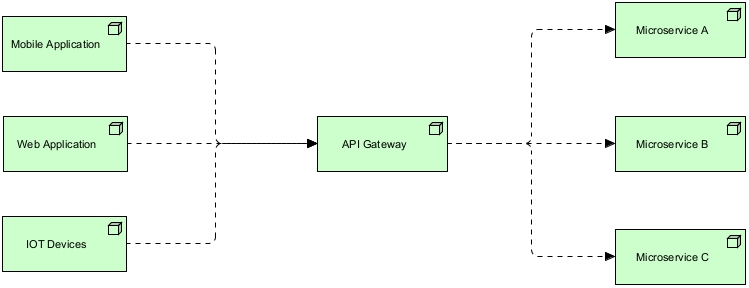
\includegraphics[width=9cm]{Media/API Gateway.jpg}
    \caption{API Gateway Pattern}
    \label{APIGATEWAY}
  \end{figure}

\end{description}


\subsubsection{Gateway Offloading}

\begin{description}
  \item[Context:] Using the same SaaS practice management system example, one can imagine that different microservices have common features and these features require maintenance, configuration and management. The features could be token validation, feature flag management, SSL certificate management, encryption or environment variable management. 
  \item[Problem:] How does one go about handling these shared features? should each team write their own feature for their own services? if a feature is updated, should each team then update their own implementation? how do we ensure that these features conform to the same interface and standards? if a new feature is added, should we communicate with three different teams to update their implementation? what happens if an implementation of on team does not respect the specification?
  \item[Solution:] Common features and cross-cutting concerns can be offloaded into a gateway. This includes but is not limited to: SSL termination, certificate management, feature flag management, environment variables management, secret management, monitoring, logging configurations, throttling, and protocol translation. This approach simplifies the development of services, and improves the maintainability of the system.  In addition, features that require special skills (privacy and security) can be developed by experts and propagated to teams, eliminating the risk that non-expert developers may introduce. This pattern also introduces more consistency, and standardised interfaces which helps with communication, agility and productivity of development teams. This pattern is portrayed at Figure ~\ref{gatewayOffloading}.   

\end{description}

\begin{figure}[h]
  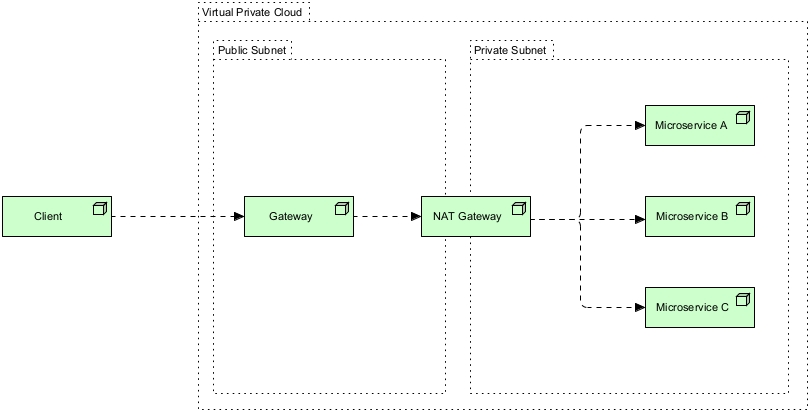
\includegraphics[width=10cm]{Media/Gateway Offloading.jpg}
  \caption{Gateway Offloading Pattern}
  \label{gatewayOffloading}
\end{figure}

\subsubsection{External configuration store}

\begin{description}
  \item[Context:] Software applications are usually deployed to various environment for different purposes. This is part of CI/CD approach that creates pipelines to capture bugs, and issues. For instance there are testing, integration, pre-production and production environments. Each environment is tailored for a different purpose. In a development environment, several features flags may be deactivated, some infrastructure may have been configured to reduce costs, and end to end tests may run. Therefore, an application needs to keep a list of configuration for internal and third-party infrastructure it needs. In addition, various class of services require radically different configurations to meet their ends. These configurations could be a buffer size setup on streaming processing services or it could be the timeout time set on batch processing services. 
  \item[Problem:] Should each application have its configuration written separately? as the number of applications grow, how does one scale and maintain this? If a configuration should be uploaded for a class of similar services, should each service update its configuration separately? how can configurations be shared across several applications? 
  \item[Solution:] Store all application configurations in an external store. This can include package versions, database credentials, network locations and APIs. On startup, application can request for the corresponding configuration from the external configuration store. This for example could happen in CMD command of Docker script. This pattern is portrated in Figure~\ref{externalConfiguration}  
\end{description}

\begin{figure}[h]
  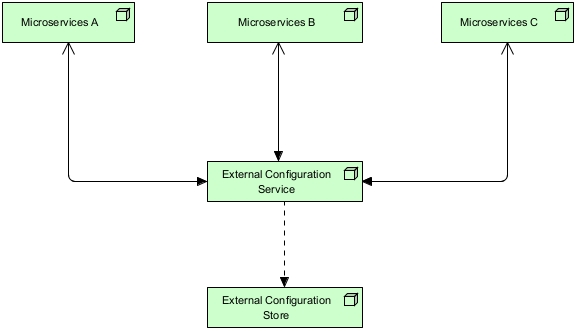
\includegraphics[width=10cm]{Media/External Configuration Store.jpg}
  \caption{External Configuration Store Pattern}
  \label{externalConfiguration}
\end{figure}

\subsubsection{Competing Consumers}

\begin{description}
  \item[Context:] An enterprise application, specially a data-intensive one is expected to handle large number of requests. Handling these requests synchronously would be challenging. A common approach is for application to send these requests through a messaging system to another application that handles them asynchronously. This ensure that one blocking service is not gonna have ripple effect on the system. Requests loads vary at different times. During peak hours there might be many requests coming from various sources. In addition, the processing required for different requests vary, and while some may be quite cheap, the other might be compute intensive. 
  \item[Problem:] Should only one consumer instance be responsible for incoming requests? what happens if that consumer instance does not have the computing resources available? what happens if that consumer instance fails? 
  \item[Solution:] Message queue system can be used to load balance requests to different consuming services based on their availability. This means that a group of consumer applications will be created, which allows in timely processing of incoming requests during peak time. This can be achieved either by a push model (message queue pushing to available consumer nodes), or a pull model (consumer nodes pull requests based on their state and process it).

  This increase the elasticity, availability and reliability of the system. The queue can act as a buffer between the producer and consumer instance, and help with minimizing the impact of consumer services unavailability. The message can also be enhanced with fault tolerant mechanisms in case of node failures. Furthermore, scalability is improved as new data consumers can be dynamically added. For instance, in AWS, auto scaling groups can be set for EC2 instances. This pattern is presented in Figure~\ref{competingConsumer}.  
\end{description}

% \paragraph{Context}

% An enterprise application, specially a data-intensive one is expected to handle large number of requests. Handling these requests synchronously would be challenging. A common approach is for application to send these requests through a messaging system to another application that handles them asynchronously. This ensure that one blocking service is not gonna have ripple effect on the system. Requests loads vary at different times. During peak hours there might be many requests coming from various sources. In addition, the processing required for different requests vary, and while some may be quite cheap, the other might be compute intensive. 


% \paragraph{Problem}

% Should only one consumer instance be responsible for incoming requests? what happens if that consumer instance does not have the computing resources available? what happens if that consumer instances fails? 


% \paragraph{Solution}

% Message queue system can be used to load balance requests to different consuming services based on their availability. This means that a group of consumer applications will be created, which allows in timely processing of incoming requests during peak time. This can be achieved either by a push model (message queue pushing to available consumer nodes), or a pull model (consumer nodes pull requests based on their state and process it).

% This increase the elasticity, availability and reliability of the system. The queue can act as a buffer between the producer and consumer instance, and help with minimizing the impact of consumer services unavailability. The message can also be enhanced with fault tolerant mechanisms in case of node failures. Furthermore, scalability is improved as new data consumers can be dynamically added. For instance, in AWS, auto scaling groups can be set for EC2 instances. This pattern is presented in Figure~\ref{competingConsumer}.

\begin{figure}[h]
  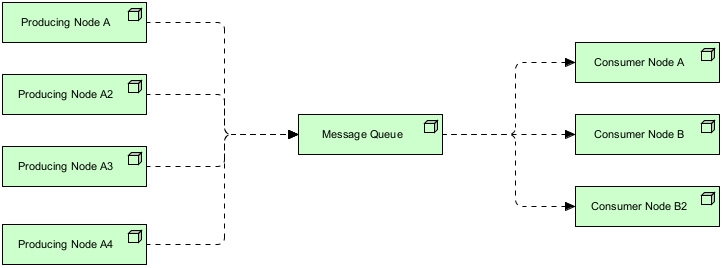
\includegraphics[width=10cm]{Media/Competing Consumers.jpg}
  \caption{Competing Consumers Pattern}
  \label{competingConsumer}
\end{figure}

\subsubsection{Circuit Breaker}

\begin{description}
  \item[Context:] Suppose a company is using a microservices architecture. There are various services that communicate with each other to process requests. If one service synchronously calls another services through a REST API, there's a chance that the other service may not be available or is exhibiting a high latency. As the number of services grow, there will be an increased requirement for communication between services. Therefore, the failure of one service can introduce a bottleneck to the whole system.
  \item[Problem:] How does one handle the failing service? how should the failed service be handled to avoid ripple effect? 
  \item[Solution:] An architect can employ the circuit breaker pattern. The circuit breaker pattern prevents services from repeatedly calling the failing service. This allows for the system to operate in spite of a failing node, which helps with saving CPU cycles, improving availability, improving reliability and decreasing the chance of faulty data. In addition, circuit breaker signals the fault resolution which allows system to get back to its default state. 

  In a common scenario, circuit breaker acts as a proxy between the source and destination services, and monitors the destination service. If the number of failing requests reach a certain threshold, the circuit breaker trips, blocking subsequent requests to the destination. The circuit breaker then probes the failing service to identify its health. Once the service becomes healthy again, the circuit breaker allows requests to be passed to the destination. 
  
  Circuit breaker can be implemented on frontend, backend, or as a standalone service. This pattern is usually implemented as a state machine that mimics the functionality of an electrical circuit breaker. This is usually designed in three states: 
  \begin{enumerate}
    \item closed: the default state, where circuit breaker listens on the number of incoming requests
    \item open: if the number of failing requests reach a certain threshold, the circuit breaker trips, immediately returning an exception
    \item half-open: a limited number of requests are passed, if these requests are passed, it is assumed that service is healthy, and circuit breaker switches to closed state. If any requests fail, the circuit breaker assumes the fault is still present, so it reverts back to open state.
  \end{enumerate}
  
  This pattern is displaed in Figure~\ref{circuitBreaker}.   
\end{description}

\begin{figure}[h]
  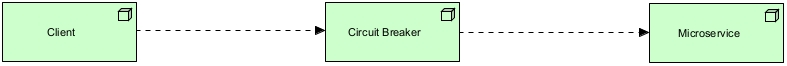
\includegraphics[width=10cm]{Media/Circuit Breaker.jpg}
  \caption{Circuit Breaker Pattern}
  \label{circuitBreaker}
\end{figure}

\subsubsection{Log Aggregation}

\begin{description}
  \item[Context:] Microservices is comprising of large set of services, each having its own domain and responsibility. A request usually spans multiple services, and in the process something might go wrong, and bugs may occur. Each system writes logs in a standardized format about errors, warning and access requests. 
  \item[Problem:] How to understand the root cause of issue if it's spanning multiple services? should one read the logs of one service, and then the logs of the other, and the next to try to make sense of the problem?  
  \item[Solution:] A centralized logging service can be implemented that retrieves logs from different services and compose them together. The developers can then search and analyze these logs to make sense of the root cause. This eliminates the tedious task of going to each service, extracting logs and aggregating them manually. This pattern is portrated in Figure~\ref{logAggregation}.    
\end{description}



\begin{figure}[h]
  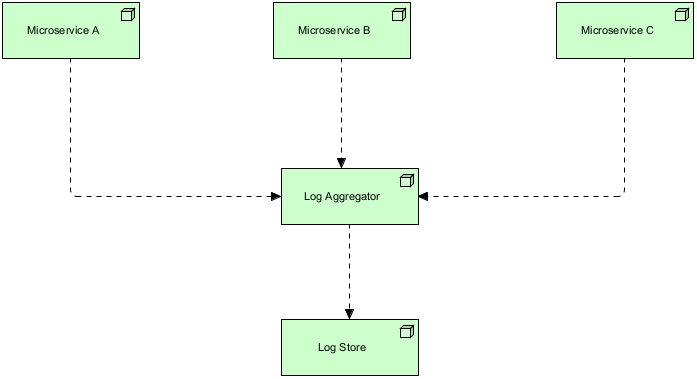
\includegraphics[width=10cm]{Media/Log Aggregation Pattern.jpg}
  \caption{Log Aggregation Pattern}
  \label{logAggregation}
\end{figure}

\subsubsection{Command and Query Responsibility Segregation}

\begin{description}
  \item[Context:] Suppose that a team is working on a data heavy service. This service needs to scale and crunch a lot of data. Following the traditional approach, often the same data model is used to query and update the database. Underlying this approach, the read and write workloads both go to the same datastore. 
  \item[Problem:] How should the team optimize for read workloads? how should the team optimize for the write workloads? can the team optimize for both read and write workloads? How does the team handle the miss match between the read and write representations of the data? how does the team ensure certain performance objective is met on read workloads?
  \item[Solution:] Implement CQRS pattern to separates reads and writes workloads, using commands to update the data and queries to read the data. This is usually achieved through a message queue asynchronously. Having the command and query separated, simplifies modeling, development and maintenance of data stores. In addition, the system will be able to support multiple denormalized views that are optimized for a specific workload. 

  CQRS is commonly implemented in two distinct data stores. This allows for the read database to optimize for read queries. For instance, it can store a materialized view of the data, and avoid expensive joints or complex ORM mappings. The read database can be a different type of data store. One might choose to use a graph database such as Neo4J for relationship heavy datasets, or a NoSQL database such as MongoDB for highly dynamic data. On the other hand, CQRS can potentially increase complexity, introduce code-duplication and increase latency. An overview of this pattern can be found at Figure~\ref{CQRS}.   
\end{description}

\begin{figure}[h]
  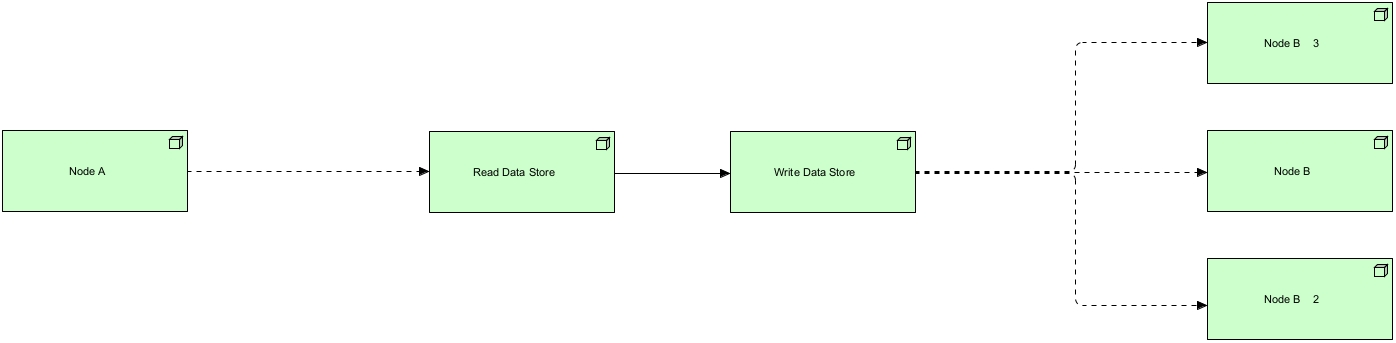
\includegraphics[width=11cm]{Media/Command and Query Responsibility Segregation.jpg}
  \caption{Command and Query Responsibility Segregation Pattern}
  \label{CQRS}
\end{figure}

\subsubsection{Anti-Corruption Layer}

\begin{description}
  \item[Context:] Most services rely on some other services for data or functionality. Each service has its own domain model. Some of these services can be external services, some of these services can be internal legacy services, and some of them can be bleeding edge services. For these services to interoperate, there is a need for a standard interface, protocol, data model or APIs.  
  \item[Problem:] How does one maintain access between legacy internal systems and bleeding edge internal systems? how does one enable interoperability between legacy internal services and external services? should the bleeding edge service be modified to account for legacy service' interface or API? should the internal services support the API requirements of external services even if they are sub-optimal? should the semantics of legacy and external services be imposed to the bleeding edge service? should services be corrupted by the requirements of other services?  
  \item[Solution:] Define an anti-corruption layer that translates semantics between different services' domains. This enables services to be unaffected by external entities, avoiding compromises on interface, design and the technological approach. Anti-corruption layer can be a module, a class inside the application or it can be an independent service. This pattern is displayed in Figure~\ref{antiCorruption}.    
\end{description}


\begin{figure}[h]
  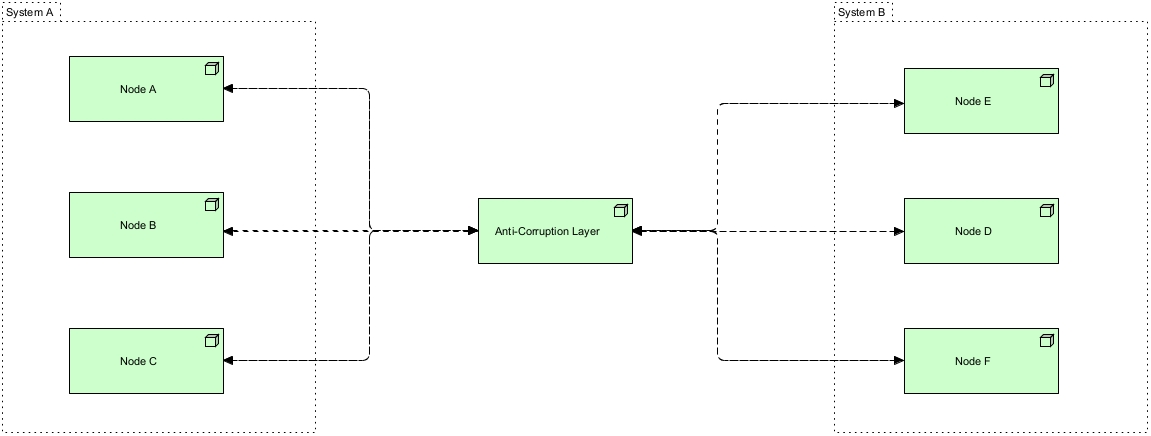
\includegraphics[width=11cm]{Media/Anti-Corruption Layer.jpg}
  \caption{Anti-Corruption Layer Pattern}
  \label{antiCorruption}
\end{figure}


\subsubsection{Backend for Frontend}

\begin{description}
  \item[Context:] In a large scale system, a backend service needs to provides the necessary APIs for various clients. A client can be the user browser, a mobile phone, or an IOT device. As the number of clients grow, the traffic grows, and new requirements emerge. As a result, the backend service needs to account for higher level of abstraction to serve the requirements of different clients. 
  \item[Problem:] Should the backend service account for various clients? if the backend service tries to account for all clients, how hard will it be to maintain this service? can a general-purpose highly abstract backend service be scaled and maintained easily? If the web development team has a conflicting requirement with the mobile development team, how does the backend service account for that? how does the backend service provide optimized data for each client? how can the backend service be optimized for various clients? 
  \item[Solution:] A dedicated backend that accounts for a specific client (frontend) can be created. This introduces opportunities for optimizing performance of each backend to best match the needs of the frontend, without worrying much about introducing side-effects to other frontends. In addition, the backend will be smaller, better abstracted, less complex, and therefore easier to maintain and scale. Furthermore, this enables horizontal teams to work without side-effects and conflicting requirements. This pattern is depicted in Figure~\ref{backend-for-fronted}.      
\end{description}

% \paragraph{Context}

% In a large scale system, a backend service needs to provides the necessary APIs for various clients. A client can be the user browser, a mobile phone, or an IOT device. As the number of clients grow, the traffic grows, and new requirements emerge. As a result, the backend service needs to account for higher level of abstraction to serve the requirements of different clients. 

% \paragraph{Problem}
% Should the backend service account for various clients? if the backend service tries to account for all clients, how hard will it be to maintain this service? can a general-purpose highly abstract backend service be scaled and maintained easily? If the web development team has a conflicting requirement with the mobile development team, how does the backend service account for that? how does the backend service provide optimized data for each client? how can the backend service be optimized for various clients? 

% \paragraph{Solution}

% A dedicated backend that accounts for a specific client (frontend) can be created. This introduces opportunities for optimizing performance of each backend to best match the needs of the frontend, without worrying much about introducing side-effects to other frontends. In addition, the backend will be smaller, better abstracted, less complex, and therefore easier to maintain and scale. Furthermore, this enables horizontal teams to work without side-effects and conflicting requirements. This pattern is depicted in Figure~\ref{BFF}.

\begin{figure}[h]
  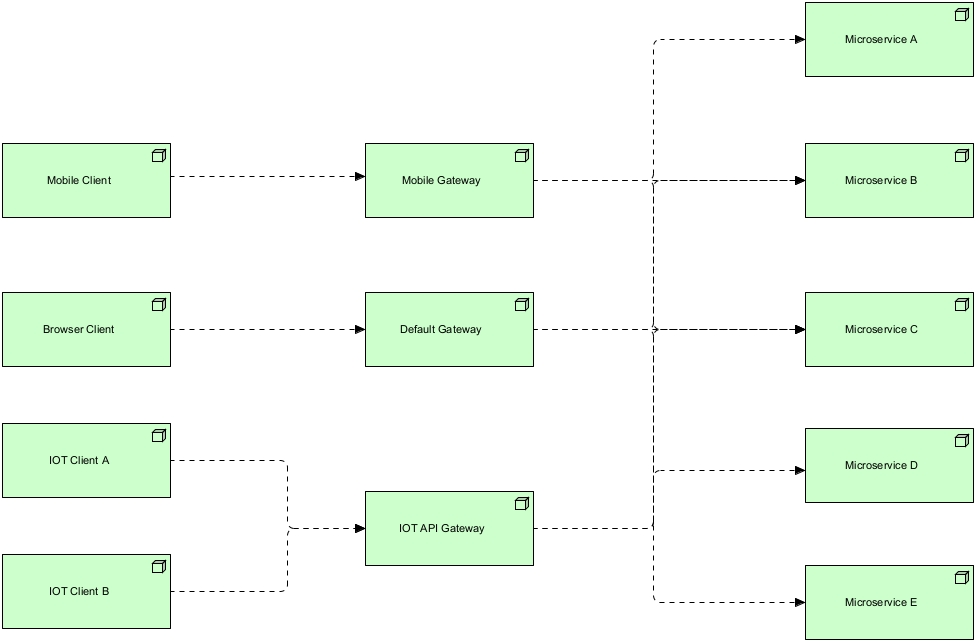
\includegraphics[width=11cm]{Media/Backend for Frontend.jpg}
  \caption{Backend for Frontend Pattern}
  \label{backend-for-fronted}
\end{figure}

\subsubsection{Pipes and filters}

\begin{description}
  \item[Context:] A large scale application is usually required to do numerous processes with varying complexity. For instance, a complex business logic may require several transformations to be done on the data. These transformations can be sophisticated and require many lines of code to be written.
  \item[Problem:] Should all these processes be performed in one monolithic module? how flexible is that approach? in light of emerging requirements how can one maintain and scale the monolithic module? is that the right level of abstraction? does this approach provide with much opportunity to optimize or reuse parts of the module? 
  \item[Solution:] Different processing can be broken down into their own components (filters), each taking a single responsibility. This provides with clean and modular components that can be extended and modified with ease. This pattern is ubiquitous in Unix like operating system; it is common for system engineers to pipe the result of the command `ls' into the command `grep' or command `sed'. By standardizing interface for data input and output, these filters can be easily combined together to create a more powerful whole. Composition then becomes natural, and maintainability increases. This pattern is portrated at Figure~\ref{PipesAndFilters}.   
\end{description}


\begin{figure}[h]
  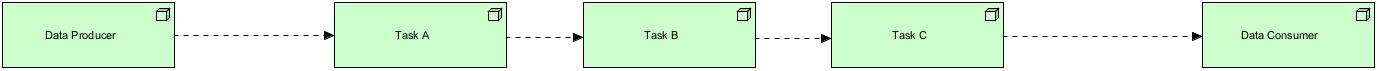
\includegraphics[width=11cm]{Media/Pipes and Filters.jpg}
  \caption{Pipes and filters Pattern}
  \label{PipesAndFilters}
\end{figure}

\section{Application of Microservices Design Patterns to Big Data Systems} \label{Mapping}


In this section, we combine our findings from both SLRs, and present new theories on application of MS design patterns for BD systems. The patterns gleaned, are established theories that are derived from actual problems in MS systems in practice, thus we do not aim to re-validate them in this study. 

The main contribution of our work is to propose new theories and try to apply some of the well-known software engineering patterns to the realm of data engineering and in specific, BD. Based on this, we map BD system requirements against a pattern and provide with reasoning on why such pattern might work for BD systems. We support our arguments by the means of modeling. We use Archimate \cite{lankhorst2013language} as recommend in ISO/IEC/IEEE 42010 \cite{Chaabane}. 

% BD systems and microservices architecture are both inherently distributed. While many of the current BD systems are designed underlying a monolithic data pipeline architecture, here, we propose microservices architecture for a domain-driven and decentralized BD architecture.

We posit that a pattern alone would not be significantly useful to a data engineering or a data architect, and propose that a collection of patterns in relation to current defacto standard of BD architectures is a better means of communication. To achieve this, we portray patterns selected for each requirement in a reference architecture. We then justify the components and describe how patterns could address the requirement. These descriptions are presented as sub section, each describing one characteristic of BD systems. 


\subsection{Volume} \label{volume}

% There has been two requirements associated to the Volume aspect of big data systems which are about handling various data types (Vol-1) and providing with a scalable storage (Vol-2). 

To address the volume requirements of BD, and in specific for Vol-1 and Vol-2 we suggest the following patterns to be effective:

\begin{enumerate}
  \item Gateway offloading
  \item API gateway
  \item External Configuration Store
\end{enumerate}

\subsubsection{API Gateway and Gateway Offloading}

In a typical flow of data engineering, data goes from ingestion, to storage, to transformation and finally to serving. However there are various challenges to achieve this process. One challenge is the realization of various data sources as described in Vol-1. Data comes in various formats from structured to semi-structured to unstructured, and BD systems need to handle different data through different interfaces. There is also streaming data that needs to be handled separately with different architectural constructs and data types. So some of the key engineering consideration for the ingestion process is that; 1) is the BD system ingesting data reliably? How frequently should data be ingested? In what volume the data typically arrives?

Given the challenges and particularities of data types, different nodes maybe spawned to handle the volume of data as witnessed in BD reference architectures studied by Ataei et al. \cite{ataei2020big}. Another popular approach is the segregation of concerns by separating batch and streaming processing nodes. Given the requirement of horizontal scaling for BD systems, it is safe to assume that there is usually more than one node associated to ingesting data. This can be problematic as different nodes will need to account for security, privacy and regional policies, in addition to the encapsulated data processing functionality. 

This means that each node needs to reimplement the same interface for the aforementioned cross-cutting concerns, which makes scalability and maintainability a daunting task. This also introduces unnecessary repetition of codes and can result in non-conforming interfaces. To solve this problem, we explore the concept of gateway offloading pattern. By offloading cross-cutting concerns that are shared across nodes to a single architectural construct, not only we will achieve a separation of concerns and a good level of usability, but we increase security and performance, by processing and filtering incoming data through a well specified ingress controller.

Moreover, if data producers directly communicate with the processing nodes, they will have to update the endpoint address every now and on. This issue is exacerbated when the data producer tries to communicate to a service that is down. Given that lifecycle of a service in a typical distributed cloud environment is not deterministic and many container orchestration systems constantly recycle services to proactively address this issue, reliability and maintainability of the BD system can be compromised. In addition, if all nodes are available externally on several ports, security management can be a daunting task. To solve these issues, the API gateway pattern can be utilized. API gateway pattern provides a single entry for data producers to communicate to internal services. The gateway can then either route incoming requests to responsible services, or it can serve as a proxy.

This layer helps decoupling data producers from the internal services, allowing for better maintainability and scalability of the BD system. In addition, the gateway can increase the system reliability and availability by doing a constant health check on services, and distribute traffic based on liveliness probes. There is also an array of other benefits such as having a weighted distribution, and creating a special cache mechanism through specific HTTP headers. This also means that if the gateway is down, service nodes won't introduce bad state into the overall system. We have portrayed a simplistic representation of this pattern in Fig \ref{fig:VolReq}. 

\subsubsection{External Configuration Store}

As discussed earlier, BD systems are made up of various nodes in order to achieve horizontal scalability. While these systems are logically separated to their own service, they will have to communicate with each other in order to achieve the goal of the system. Thus, each one of them will require a set of runtime environmental configuration. 

These configurations could be database network locations, feature flags, and third party credentials. Moreover, different stages of the data engineering may have different environments for different purposes, for instance, privacy engineers may require a completely different environment to achieve their requirements. Therefore, the challenge is the management of these configurations as the system scales, and enabling services to run in different environments without modification. To address this problem, we propose the external configuration store pattern.

By externalizing all nodes configuration to another service, each node can request its configuration from an external store on boot up. This can be achieved in Docker files through the CMD command, or could be written in Terraform codes for a Kubernetes pod. This pattern solves the challenges of handling large number of nodes in BD systems and provide with a scalable solution for handling configurations. This pattern is portrayed in Fig \ref{fig:VolReq}.

\begin{figure*}[h]
    \centering 
    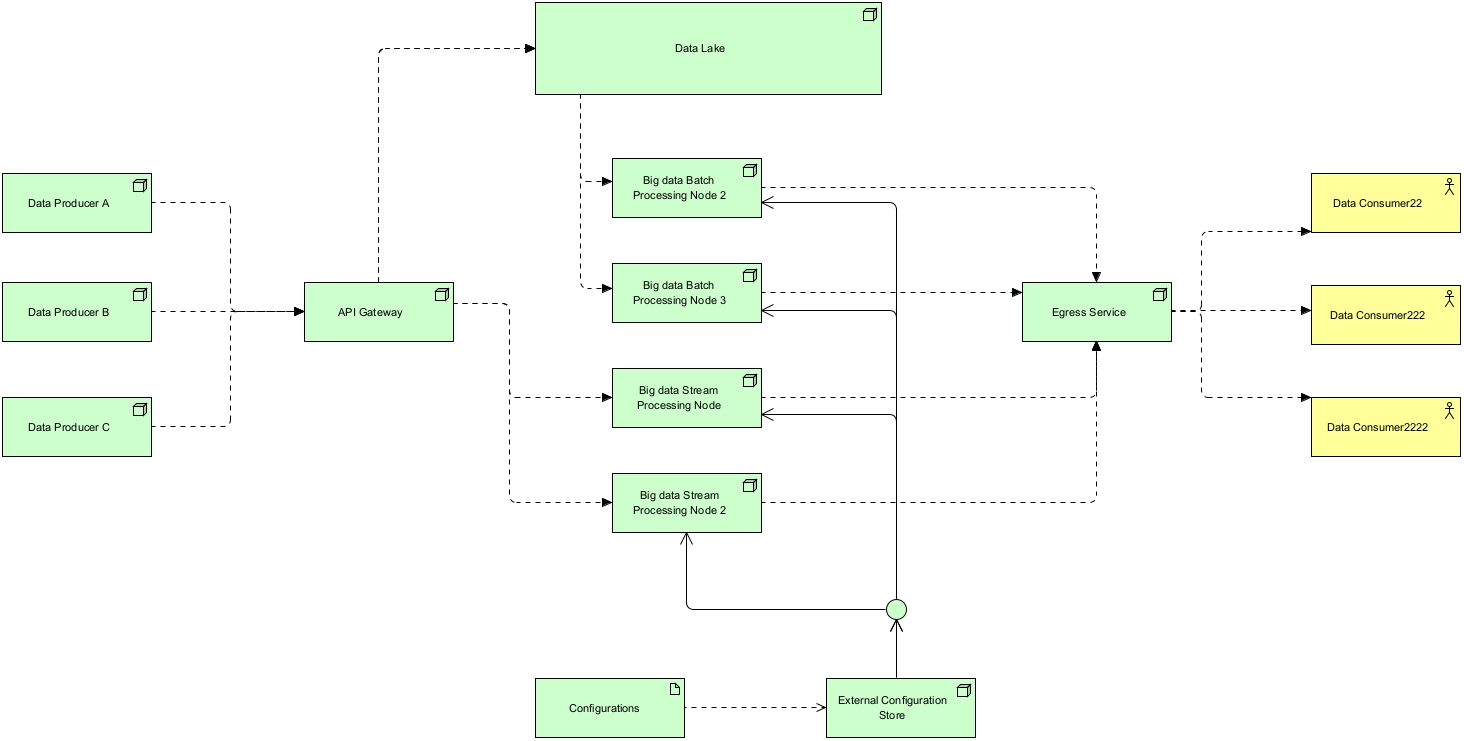
\includegraphics[width=12cm]{Media/Vol-1 Requirement RA.jpg}
    \caption{Microservices Patterns for BD Volume Requirements}
    \label{fig:VolReq}
\end{figure*}

\subsection{Velocity}

Velocity is perhaps one of the most challenging aspects of the BD systems, which if not addressed well, can result in series of issues from system availability to massive loses and customer churn. To address some of the challenges associated with the velocity aspect of BD systems, we recommend the following patterns for the requirements Vel-1, Vel-2, Vel-3, and Vel-5:


\begin{enumerate}
  \item Competing Consumers
  \item Circuit Breaker
  \item Log Aggregation
\end{enumerate}


\subsubsection{Competing Consumers}

BD doesn't imply only 'big' or a lot of data, it also implies the rate at which data can be ingested, stored and analyzed to produce insights. According to a recent MIT report in collaboration with Databricks, one of the main challenges of BD 'low-achievers' is the 'slow processing of large amounts of data' \cite{DataBricksSurvey}. If the business desires to go data driven, it should be able to have an acceptable time-to-insight, as critical business decisions cannot wait for data engineering pipelines. 

Achieving this in such a distribute setup as BD systems with so many moving parts, is a challenging task, but there are MS pattern that can be tailored to help with some of these challenges. Given the very contrived scenario of a BD system described in the previous section, at the very core, data needs to be ingested quickly, stored in a timely manner, micro-batch, batch, or stream processed, and lately served to the consumers. So what happens if one node goes down or becomes unavailable? in a traditional Hadoop setup, if Mesos is utilized as the scheduler, the node will be restarted and will go through a lifecycle again. 

This means during this period of time, the node is unavailable, and any workload for stream processing has to wait, failing to achieve requirements Vel-2, Vel-3 and Vel-5. This issue is exacerbated if the system is designed and architected underlying monolithic pipeline architecture with point-to-point communications. One way to solve some of these issues, is to introduce an event driven communication as portrayed in the works of Ataei et al. \cite{ataei2021neomycelia}, and try to increase fault tolerance and availability through competing consumers, circuit breaker, and log aggregation. 

Underlying the event-driven approach, we can assume that nodes are sending each other events as a means of communication. This implies that node A can send an event to node B in a 'dispatch and forget' fashion on a certain topic. However this pattern introduces the same problem as the point-to-point REST communication style; if node B is down, then this will have a ripple effect on the whole system. To address this challenge, we can adopt the competing consumer pattern. Adopting this pattern means instead of one node listening on the topic, there will be a few nodes. 

This can change the nature of the communication to asynchronous mode, and allow for a better fault tolerance, because if one node is down, the other nodes can listen to the event and handle it. In other terms, because now there are a few consumers listening on the events being dispatched on a certain topic, there's a competition of consumers, therefore the name 'competing consumers'. For instance, three stream processing consumer nodes can be spawned to listen on data streaming events being dispatched from the the up-stream. This pattern will help alleviate challenges in regards to Vel-2, Vel-3 and Vel-5.

\subsubsection{Circuit Breaker}

On the other hand, given the large number of nodes one can assume for any BD system, one can employ the circuit breaker pattern to signal the service unavailability. Circuit breakers can protect the overall integrity of data and processes by tripping and closing the incoming request to the service. This communicates effectively to the rest of the system that the node is unavailable, allowing engineers to handle such incidents gracefully. This pattern, mixed with competing consumers pattern con increase the overall availability and reliability of the system, and this is achieved by providing an even-driven asynchronous fault tolerance communication mechanisms among BD services. This allows system to be able to be resilient and responsive to bursty, high-throughput data as well as small, batch oriented data, addressing requirements Vel-1, Vel-4, and Vel-5. 
    
\subsubsection{Log Aggregator}

Given that BD systems are comprising of many services, log aggregation can be implemented to shed lights on these services and their audit trail. Traditional single node logging does not work very well in distributed environments, as engineers are required to understand the whole flow of data from one end to another. To address this issue, log aggregation can be implemented, which usually comes with a unified interface that services communicates to and log their processes from. This interface then, does the necessary processes on the logs, and finally store the logs. 

In addition, reliability engineers can configure alerts to be triggered underlying certain metrics. This increases teams agility to proactively resolve issues, which in turn increases reliability and availability which in turn addresses the velocity requirement of BD systems. While this design pattern does not directly affect any system requirements, it indirectly affects all of them. A simplistic presentation of this pattern is portrayed in Fig \ref{fig-vel-ra}. 


\begin{figure*}[h!]
    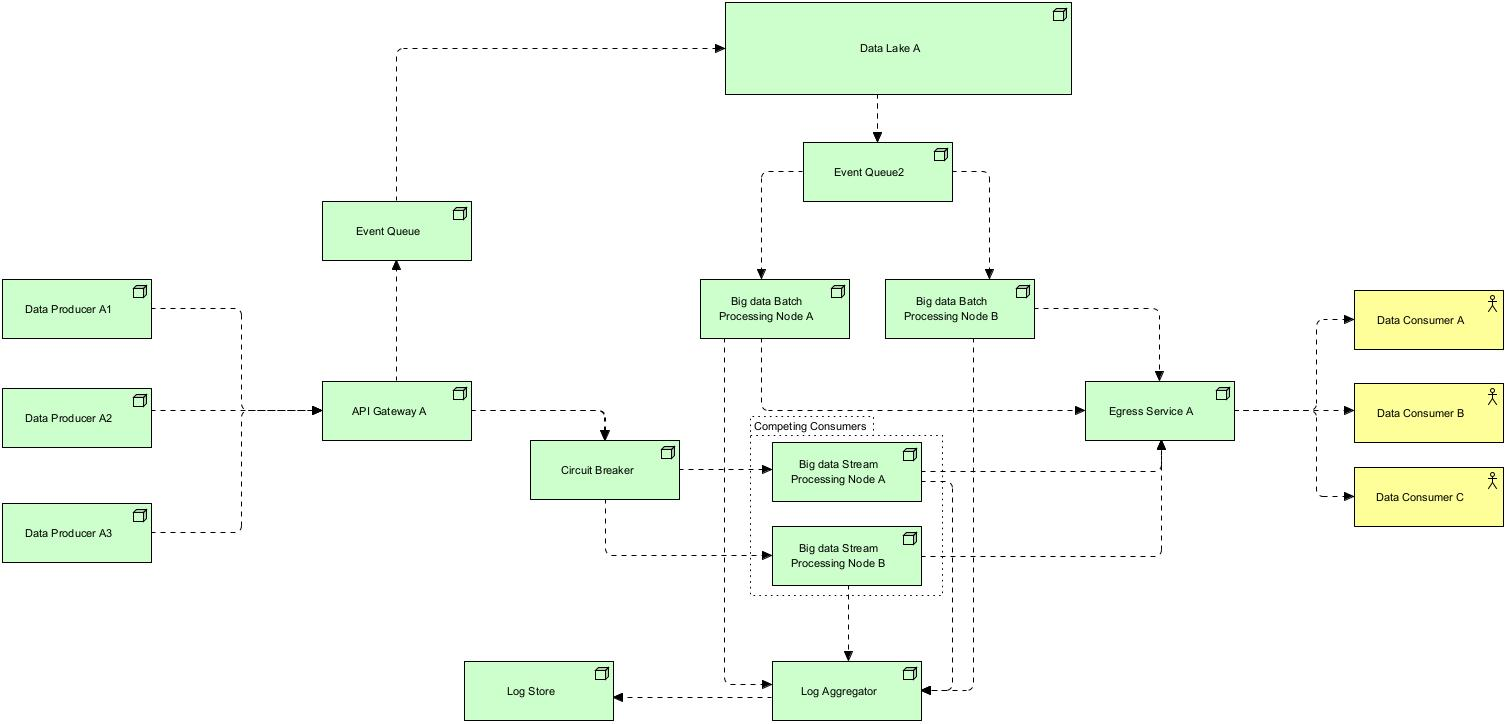
\includegraphics[width=12cm]{Media/Velocity Requirement.jpg}
    \caption{Design patterns for velocity requirements}
    \label{fig-vel-ra}
\end{figure*}


\subsection{Variety}

Variety, being another important aspect of BD, implies the range of different data types and the challenges of handling these data. As BD system grows, newer data structures emerge, and an effective BD system must be elastic enough to handle various data types. To address some of the challenges of this endeavour, we recommend the following patterns to address requirements Var-1, Var-3, Var-4:

\begin{enumerate}
  \item API Gateway
  \item Gateway Offloading
\end{enumerate}


\subsubsection{API Gateway and Gateway Offloading}

We have previously discussed the benefits of API Gateway and Gateway Offloading, however in this section we aim to relate it more to BD system requirements Var-1, Var-3, and Var-4. Data engineers need to keep an open line of communication to data producers on changes that could break the data pipelines and analytics. Suppose that developer A changes a field in a schema of an object that may break a data pipeline or introduce a privacy threat. How can data engineers handle this scenario effectively? 

To address this problem, API Gateway and Gateway Offloading can be used. API Gateway and Gateway Offloading could be good patterns to offload some of the light-weight processes that maybe associated to the data structure or the type of data. For instance, a light weight metadata check or data scrubbing can be achieved in the gateway. However, Gateways themselves should not be taking a lot of responsibility and become a bottleneck to the system. Therefore, as nodes increase and requirements emerge, one might chose to opt for 'Backend for Frontend' pattern. We do not do any modeling for this section, as the high-level overview of API Gateway pattern is portrayed in Figure \ref{fig:VolReq}.

\subsection{Value}

Value is the nucleus of any BD endeavour. In fact all components of the system pursue the goal of realizing a value, that is the insight derived from the data. Howbeit, realizing these insights require absorption of great deal of complexity. To address some of these challenges, we propose the following patterns to address the requirements Val-1, Val-3, and Val-4:

\begin{enumerate}
  \item Command and Query Responsibility Segregation (CQRS)
  \item  Anti-Corruption Layer
\end{enumerate}

\subsubsection{Command and Query Responsibility Segregation}

Suppose that there are various application that would like to query data in different ways and with different frequencies (Val-3, Val-4). Different consumers such as business analysts and machine learning engineers have very different demands, and would therefore create different workloads for the BD systems. As the consumers grow, the application has to handle more object mappings and mutations to meet the consumers demands. This may result in complex validation logics, transformations, and serialization that can be write-heavy on the data storage. As a result the serving layer can end up with an overly complex logic that does too much. 

Read and write workloads are really different, and this is something a data engineer should consider from the initial data modeling, to data storage, retrieval and potential serialization. And while the system may be more tolerant on the write side, it may have a requirement to provide reads in a timely manner (checking a fraudulent credit card). Read and write representation of the data are often different and miss-matching and require a specific approach and modeling. For instance a snowflake schema maybe expensive for writes, but cheap for reads. 

To address some of these challenges, we suggest CQRS pattern. CQRS separates the read from writes, using commands to update the data, and query to read data. This implies that the read and write databases can be physically segregated and consistency can be achieved through an event. To keep databases in sync, the write database can publish an event whenever an update occurs, and the read database can listen to it and update its values. This allows for elastic scaling of the read nodes, and increased query performance. This also allows for a read optimized data modeling tailored specifically for data consumers. Therefore, this pattern can potentially address the requirement Val-1, and Val-3. 

\subsubsection{Anti-Corruption Layer}

Another pattern that comes useful when handling large number of data consumers is the anti-corruption layer. Given that the number of consumers and producers can grow and data can be created and requested in different formats with different characteristics, the ingestion and serving layer may be coupled to these foreign domains and try to account for an abstraction that aims to encapsulate all the logic in regards to all the external nodes. As the system grows, this abstraction layer becomes harder to maintain, and its maintainability becomes more difficult. 

One approach to solve this issue is anti-corruption layer. Anti-corruption layer is a node that can be placed between the serving layer and data consumers or data producer, isolating different systems and translating between domains. This eliminates all the complexity and coupling that could have been otherwise introduced to the ingestion layer or the serving layer. This also allows for nodes to follow the 'single responsibility' pattern. Anti-corruption layer can define strong interfaces and quickly serve new demands without affecting much of the serving node's abstraction. In another terms, it avoids corruption that may happen among systems, by separating them. This pattern can help with requirements Val-3 and Val-4. We have portrayed this pattern and CQRS in Figure \ref{fig:Value Requirements}.

\begin{figure*}[h]
    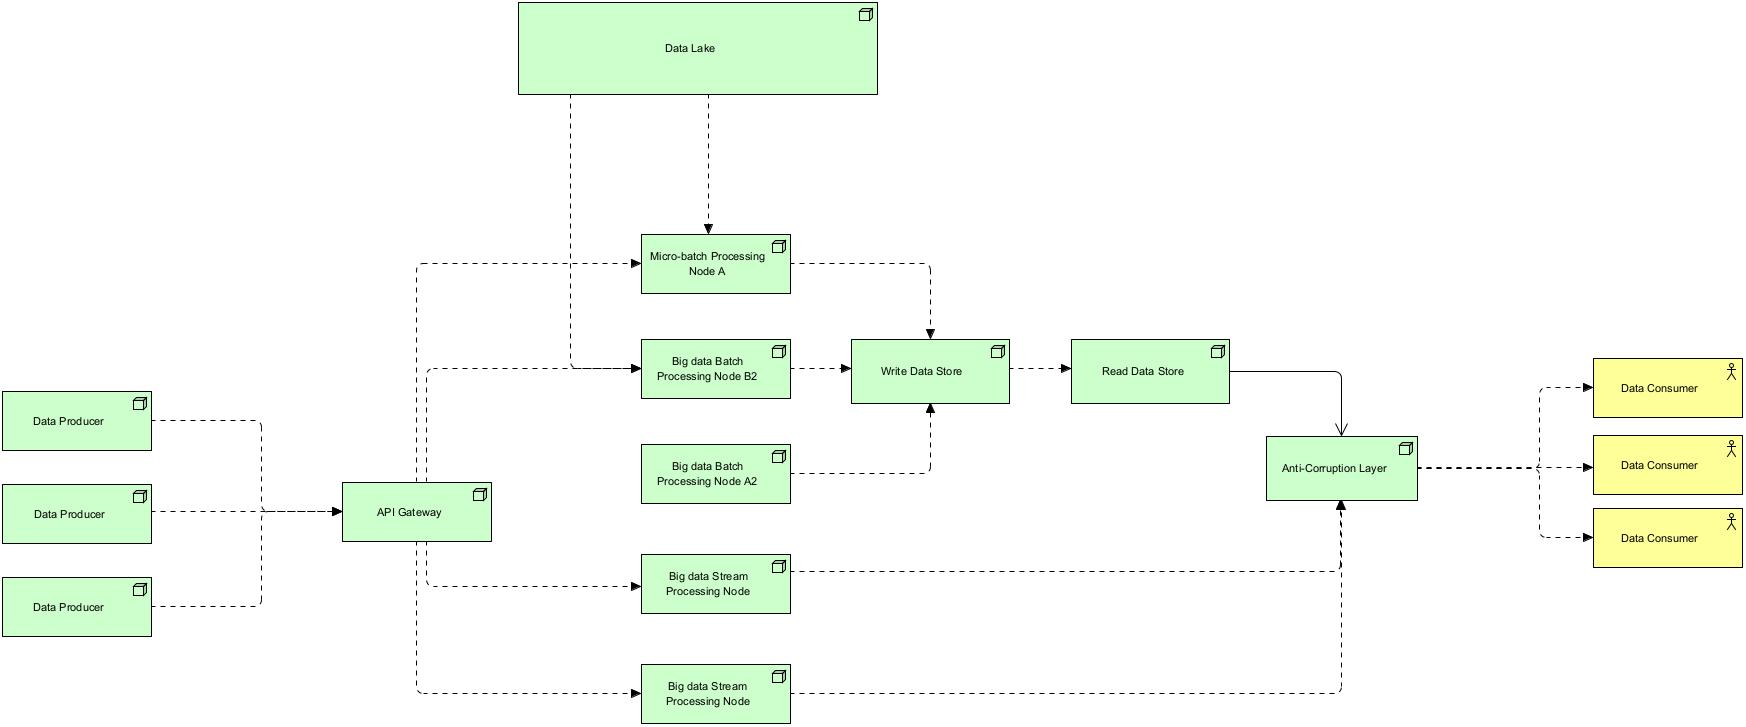
\includegraphics[width=12cm]{Media/Value Requirement.jpg}
    \caption[]{Design patterns for value requirement }
    \label{fig:Value Requirements}
\end{figure*}

\subsection{Security and Privacy}

Security and privacy should be on top of mind for any BD system development, as these two aspects play an important role in the overall data strategy and architecture of the company. At the intersection of data evolution, regional policies, and company policies, there's a great deal of complexity. To this end, we propose the following pattern to address requirements SaP-1 and SaP-2:

\begin{enumerate}
  \item Backend for Frontend (BFF)
\end{enumerate}

\subsubsection{Backend for Frontend}

API gateway has been discussed in several sections in this study, however, in this section we are interested to see how it can improve security and privacy of BD systems. In terms of privacy, given the increasing load of data producers, and how they should be directed to the right processing node, how does one comply with regional policies such as GDPR? how do we ensure, for example, that data is anonymized and identifiable properties are omitted? one approach is to do this right in the API gateway. However as data consumers grow and more data gets in, maintaining the privacy rules and applying them correctly to the dataset in the API gateway becomes more difficult. In addition, this can result in a bloated API gateway with many responsibilities, that can be a potential bottleneck to the system.

On approach to this problem can be the BFF pattern. By creating backends (services) for frontends (data producers), we can logically segregate API gateways for data that requires different level of privacy and security. This logical separation can include other factors such as QoS, key accounts, and even the nature of the API (GraphQL or RPC). Implementing this pattern means that instead of trying to account for all privacy related concerns in one node (API gateway), we separate the concerns to a number of nodes that are each responsible for a specific requirement. This means, instead of creating a coupled, loosely abstracted implementation of privacy mechanisms, the system can benefit from hiding sensitive or unnecessary data in a logically separated node. This is also a great opportunity for data mutation, schema validation, and potentially protocol change (receive REST, and return GraphQL).

On the other hand, from the security point of view, and in specific in relation to authorization and authentication, this pattern provides with a considerable advantage. BFF can be implemented to achieve token isolation, cookie termination, and a security gate before requests can reach to upstream servers. Other security procedures such as sanitization, data masking, tokenization, and obfuscation can be done in this layer as well. As these BFF servers are logically isolated for specific requirements, maintainability and scalability is increased. This addresses the requirements SaP-1 and SaP-2. We have modeled this pattern in Figure~\ref{fig:SaP Requirements}

\begin{figure*}[h]
  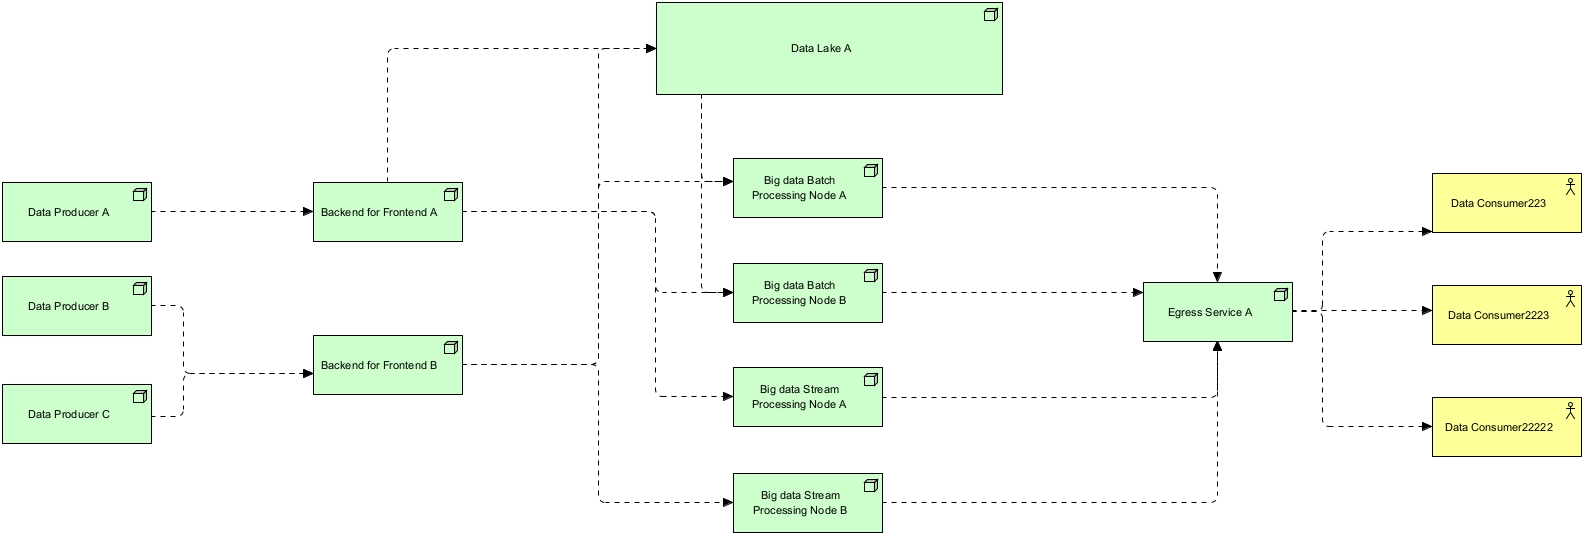
\includegraphics[width=12cm]{Media/Privacy and Security Requirements.jpg}
  \caption[]{Design patterns for security and privacy requirements}
  \label{fig:SaP Requirements}
\end{figure*}


\subsection{Veracity}

Next to value, veracity is an integral component of any effective BD system. Veracity in general is about how truthful and reliable data is, and how signals can be separated from the noises. Data should conform with the expectations from the business, thus data quality should be engineered across the data lifecycle. According to Eryurek et al. \cite{eryurek2021data}, data quality can be defined by three main characteristics 1) accuracy, 2) completeness, and 3) timeliness. Each of these characteristics posit a certain level of challenge to architecture and engineering of BD systems. To this, we propose the following patterns for addressing requirements Ver-1, and Ver-4:

\begin{enumerate}
  \item Pipes and filters 
  \item Circuit breaker
\end{enumerate}


\subsubsection{Pipes and Filters}

Suppose that there is a data processing node that is responsible for performing variety of data transformation and other processes with different level of complexities. As requirements emerge, newer approaches of processing may be required, and soon this node will turn into a big monolithic unit that aims to achieve too much. Furthermore, this node is likely to reduce the opportunities of optimization, refactoring, testing and reusing. In addition, as the business requirements emerge, the nature of some of these tasks may be different. Some processes may require a different metadata strategy that requires more computing resources, while others might not require such expensive resources. This is not elastic and can produce unwanted idle times. 

One approach to this problem could be the pipes and filters pattern. By implementing pipes and filters, processing required for each stream can be separated into its own node (filter) that performs a single task. This is a well-established approach in unix-like operating systems. Following this approach allows for standardization of the format of the data and processing required for each step. This can help avoiding code duplication, and results in easier removal, replacement, augmentation and customization of data processing pipelines, addressing the requirements Ver-1 and Ver-4. This pattern is basically portrayed in all of our models.

\subsubsection{Circuit breaker}
 
In an inherently distributed environment like BD, calls to different services may fail due to various issues such as timeouts, transient faults or service being unavailable. While these faults may be transient, this can have a ripple effect on other services in the system, causing a cascading failure across several nodes. This affects system availability and reliability and can cause major losses to the business. 

One solution to this problem can be the circuit breaker pattern. Circuit breaker is a pattern that prevents an application from from repeatedly trying to access a service that is not available. This improves the fault tolerance among services, and signals the service unavailability. The requesting application can decide accordingly on how to handle the situation. In other terms, circuit breakers are like proxies for operations that might fail. This proxy is usually implemented as a state machine having the states close, open, and half-open. Having this proxy in place provides stability to the overall BD system, when the service of interest is recovering from an incident. This can indirectly help with Ver-4. We have portrayed this pattern in Figure~\ref{fig-vel-ra}.


% % Pouya

\section{Validation}

After the generation of the design theories, we sought for a suitable model of validation. This involved a thorough research in some of the well-established methods for validation such as single-case mechanism experiment, technical action research and focus groups \cite{wieringa2014design}. For the purposes of this study we chose semi-structured interviews (SSIs), following the guidelines of Kallio et al. \cite{kallio2016systematic}. 



\subsection{Interview design}
Our SSI methodology is made up of four phases: 1) identifying the rationale for using semi-structured interviews, 2) formulating the preliminary semi-structured interview guide, 3) pilot testing the interview guide, 4) presenting the results of the interview. 

SSI are suitable for our study, because our conceptual framework is made up of architectural constructs that can benefit from in-depth probing and analysis. As we examine an uncharted territory with a lot of potential, we posit that these interviews can post useful leads which we can pursue to further improve the theories of this study.

 We've formulated our SSI guide based on our research objective to achieve the richest possible data. Our guide is flexible, to increase our opportunity to explore new ideas, and allow for participant-orientation. Nevertheless, we do have some close-ended questions at the start of our interview which is a good starter, and also helps us with some statistics. 

Our questions are categorized into main themes and follow-up questions, with main themes being progressing and logical, as recommended by Kallio et al. \cite{kallio2016systematic}. We pilot tested our interview guide using internal testing, which involved an evaluation of the preliminary interview guide with the members of the research team. We aimed to assume the role of the interviewee and gain insight into the limitations of our guide.

This approach helped us capture some issues with the questions, and remove some questions that may be deemed eccentric. Follow-up questions were utilized to direct the dialogue towards the subject of our study, and make things easier for candidate to understand. Some of these follow-up questions were improvised, as we did not aim to rigidly control the flow of the interview. After this, to ensure the rigour and relevance of the interview guide, we've conducted a pilot test. This step was necessary to make informed adjustments to the guide, and to improve quality of data collection. 


\subsection{Sampling strategy}

After having our interview guide designed, we used purposive sampling \cite{baltes2022sampling} to select experts. We chose purposive sampling because it allowed us to collect rich information by expert sampling. In addition, this approach enabled us to ensure representativeness and removed the need for a sampling frame. We also attempted `heterogeneity sampling' by approaching candidates from various industries. 

We reached out to colleagues, our connections on ResearchGate and Linkedin, and tried to look for experts with the titles 'data engineer', 'data architect', 'senior data engineer', 'solution architect', 'lead architect', and 'big data architect'. We also included founders of big data companies, or academics who have been working on BD systems. We interviewed 6 experts from various industries over a period of 3 months. An overview of these experts are portrayed in Table~\ref{interviewees}. 


\begin{table}[h]
  \renewcommand{\arraystretch}{1.5}
  \caption[]{Participants Demographics}
  \begin{tabular}{|p{1.4cm}|p{4cm}|p{1.5cm}|p{2.5cm}|}
      \hline
      interviewee & Role & Years of Experience  & Industry \\  

      \hline
      i1 & Lead Development Architect & 18 &  Healthcare Diagnostic Substances \\   
      \hline
      i2 & Software Architect & 8 &  Human Resources Services  \\   
      \hline
      i3 & Associate Professor and Co-founder of a Big Data company & 15 &  Consulting \\   
      \hline
      i4 & Senior Data Engineer & 20 &  Software (Practice Management Software) \\   
      \hline
      i5 & Big Data Architect & 8 &  Insurance and Finance \\   
      \hline
      i6 & Director & 40 &  Consulting \\   
      \hline
      i7 & Solution Architect & 9 &  Telecommunications \\   
      \hline
      
  \end{tabular}
  \label{interviewees}
\end{table}


\subsection{Data Synthesis}

All the interviews have been done through the software Zoom. We saved all of the recordings, and then downloaded the automatically generated transcripts. Transcripts for each interview has been added to Nvivo and then codes are created. We created a code for each BD characteristics discussed in Section~\ref{requirementSpec}. Additionally, we added a code named 'comments/suggestions'. After having analyzed all the transcripts, we added a new code named 'limitation'. This last code discussed how some of patterns of microservices may not be relevant at all, or some of the patterns we proposed may introduce challenges. 

After the initial coding process, through axial coding, we created higher level codes. These higher level codes were connected to create themes. 


\subsection{Results}

From the results of these interviews, we gathered a lot of insights and probed deep into our architectural constructs. Every interview involved in deep analysis of the design patterns with one question from the interviewee trying to understand the problem space and solution better. Our interviewees had at least 8 years of experience. While some of our interviewees had more experience with BD and AI, some others were well-versed in MS architecture. We first asked interviewees about their depth of understanding with MS and BD, and then asked them if patterns discussed for each characteristic makes sense. We asked every interviewee if they can think of a pattern that we failed to consider. Our interview guide is available at Appendix~\ref{interviewGuide}. While we designed the interview to be only an hour, the interview has always exceeded this time. We present the result of the interviews in sub-section each associated to the corresponding BD characteristic.



\subsection{Volume}

For volume, we went through the theories elaborated in Section~\ref{volume}. This was accompanied by the model created, and sometimes even live modeling to help with understanding. All of the interviewees took the idea of API gateway and gateway offloading naturally, while we had to explore the 'external configuration store' a bit deeper. We used the idea of Kubernetes ingress to help with elaboration of API gateway. We used AWS load balancer example, and discussed the challenges of maintaining certificates and authentication. For the externalized configuration pattern we had to go a bit deeper and talk about a scenario in a which the developer of the batch processing node or the stream processing node, may need to account for the development, trial and production workloads that have different DNS requirements, and configurations. We discussed how environment variables may vary, have development and trial environments may not need as much resources as the production, how ingress may vary, how recursive DNS resolution would be different, and how buffers, and hardware may vary. 

After explaining a scenario, interviewees agreed that this pattern can help with some of the challenges of data engineering. One interviewee mentioned that this can even be utilized for special privacy requirements. That is, different nodes may have different configuration based on the privacy policies needed. In addition, there's been discussion in regards to regional privacy and security requirements and how configuration can help derive them. Some interviewees discussed that this is a general pattern that any system can utilize to its benefit. 

In one interview, an interviewee discussed how the description of these patterns and the implementations varied in his professional experience in different companies. He added that most developers tend to have a shallow understanding of why certain pattern is adopted, and thus the implementation usually varies. In addition, the interviewee stated that once a pattern is implemented, then the challenge is to keep the pattern comply with its intended responsibility. In his experience, many of the patterns such as API gateway suddenly turn into an overarching solution that aims to solve many problems. Thus, patterns may firmly establish the problem domain and the solution initially. Then, too, they may emerge into something complicated different to account for newer problems. 

Another interviewee discussed how they are taking extensive measures to embark on a fully event-driven process, and how a lot of things that we theorize and modeled may sound easy to do, but daunting to implement. The interviewee explained how they are planning to store data in their AWS S3 initially and then having a Lambda function trigger to start the ETL process. The interviewee then explained how they need to obtain different configurations from different data providers, and how that can affect the data prepared for data consumers. He discussed an archetype in which the data would be stored in AWS S3, which triggers a Lambda function to initial an ETL process. Furthermore, he added how externalized configuration pattern could be implemented with DynamoDB and Lambda functions.

One of the interviewees from insurance and finance sector mentioned that scaling the gateway and corresponding nodes may not be as easy as it seems. He mentioned that during normal days there are hardly any claims, and while there's a special event, the storm comes. The interviewee mentioned that scaling forecast is usually based on historical data. Further, he mentioned that even the delay in auto-scaling groups in AWS can be problematic for them. 

The same interviewee from the insurance sector discussed how centralizing configuration may sound like a good idea. Howbeit, he added that this approach makes him slightly nervous, because every service is unique in its own, and may require a specific configuration. He added, that as configurations store, the externalized configuration node can be bloated, taking so much responsibilities. He added that at times, his team had to reconfigure a service at the fly to prevent customer churn, and with this pattern he finds everything more complicated. At last, he added that in a multi-region operating companies, a centralized configuration store can really help with standardization and maintenance. 


Another interiveee from the financial sector has affirmed us that gateway offloading and API gateways are pretty common patterns, and he has witnessed it in several major banks. The same candidate has elaborated that `external configuration store' pattern is sometimes referred to as `declarative configuration management'. The candidate then continued to explain how this pattern can be witnessed in Kubernetes clusters through metadata objects, kube-system and Etcd.


\,

\setlength{\fboxsep}{0.7em}
\noindent\fbox{%
    \parbox{\textwidth}{%
       Gateways are useful constructs. External configuration store can help alleviate challenges with distributed systems in multi-environment multi-region setups. 
    }%
}


\subsection{Velocity}

For Velocity, we first started by exploring an event-driven data engineering architecture, and then justified the idea of competing consumers. We then explored how competing consumers can fail, and how circuit breaker pattern can help. Finally we explore the idea of logging and how tail logging and distributed tracing can be achieved through it. An interviewee challenged the idea of competing consumer and stated that a leader election may be a better choice for a distributed setup as such. The interviewee also mentioned that circuit breakers could be implemented on the competing consumers themselves, but he could see the value of separating it to its own service. Of particular argument was the fact that circuit breaker's implementation may not be that complicated and a dedicated service for it can increase costs.  

In another interview, interviewee asked about the amalgamation technique for the logs, and discussed how dimensionality of the logs can be challenging. We took both feedbacks of 'leader election' and 'more in-detailed logging approach' into consideration. We researched deeper into leader election, logging approaches, and distributed tracing. We found leader election a bit hard to justify, as it introduces a single point of failure, can potentially introduce faulty data as there's only one point of trust, and partial deployments are really hard to apply. We found that benefits of 'leader election' pattern to be outweighed by the complexity it introduces. In regards to logging, we found various approaches to distributed tracing and log merging, however these were mostly in-detailed micro approaches, which is not in the scope of our study. 

In another interview, the interviewee discussed how circuit breakers may need to do load balancing as well. We then discussed how circuit breakers could be implemented in data processing nodes themselves, or in a side car. The interviewee then explained how they've created a system that resembles to the log aggregator pattern. The interviewee elaborated how the system has a graphical interface that captures errors from various ETL jobs. 

An interviewee from the insurance sector discussed how log aggregator might be a good pattern, but it's not always great to add so many technologies to the stack. Then he added that each system may have a different logging library and interface and aggregating them may need an effective methodology. The interviewee described that logging is better be approached through several layers of abstraction. He described how it would be useful to have some easy to understand metrics on the surface level. He added there should not be a need for technical skills to read these metrics. Nevertheless, there should be detailed logs abstracted for more technical users.

Moreover, it was mentioned that only important pieces of information should be collected and presented, as most web servers such as Nginx create so many logs. 

In an another interviewee, the candidate brough to light the challenges of time-sychroonization in log aggregator pattern. The candidate, who had a background in financial sector, discussed how handling logs from a large amount of can introduce a challenge of its own. He continued to describe how critical these logs can be during sensitive stream processing tasks, and how data can easily get into petabytes in the banks. 

The candidate recommended to design services in a manner that promotes self-awareness. This is to prevent them from breaking silently, which makes debugging and issue resolution much longer. He added that this 'awareness' can be complementary to log aggregator, as services can reflect and dispatch an event in regards to the root cause of the failure. In addition, the candidate discussed the benefits of dynamically defining the level of logging. 

He illustrated how dynamically setting the level of logging has been really helpful in his personal experience. The candidate then explore further on low-level technical details of implemeting OpenTelemtry for different cases and with different level of logging.  

An interviewee from the telecommunication domain decpited the fact that signaling unavailability through a circuit breaker would not suffice. The candidate continued discussing that even when services are down, you would still like to keep the data to be processed later. The candidate discussed that services to processes the data may fail, and you may even signal the data producers. But that does not mean that data producers will stop sending you data! He continued discussing how data coming from the producers may be perceived as one commit from system's and application point of vview, and how sometimes there's no way to stop the data from getting into the system. 

Therefore, he suggested that during the failure the incoming data should be stored somewhere to be processed later. In his experience, without this, things would become really challenging and there might even be a data loss. Candidate believed that data producers are hardly controlled by the data engineering pipelines and therefore data architect should adopt the approach of 'zero expectation from data producers'. He then continued discussing how his team has been handling these situations in Kafka, and how partitions have helped with consistency through offsets. 


\subsection{Variety}

For variety, we discussed common data types that need support, and how system may use parquet, JSON, or how unstructured data can introduce challenges. By this point, interviewees had a better grasp of our models and the gateway patterns, thus there wasn't much questions. An interviewee suggested the 'API composition' pattern and suggested that we may have various services that handle different data types, but the composition of these data may be necessary. The interviewee suggested that 'API composition' can occur at the egress level. 

One interviewee provided details on how painful it has been for his team to onboard new data producers and how that dramatically slowed the project deadline. The interviewee added that data received from data producers hardly have the standards necessary, as these data are generated by third-party software that they have no control over. He explained how different versions of the same software create different schema and how this can sometimes break the data engineering pipelines. Then, the interviewee suggested off-loading more compute intensive checks to gateways. We discussed how that could result in a bloated architectural construct and both parties decided that BFF pattern is probably a better suit.  

Another interviewee from insurance sector discussed how the rate of change is very low and most things are standard in insurance and finance sectors. For instance, he stated that if Avro is being used as the data format, the industry will be using the same format for the next 5 years. Additionally, the interviewee explained breaking that changes, specially schema changes are usually avoided. He added that in German insurance companies, almost everything is standard, and introducing any change would require large scale communication with all insurance companies which is an extensive measure. 

One of the participants who had an experience with firmware development, depicted the challenges of working with Eletronic Data Interchange (EDI) formats. In his experience the data format has hardly changed despite the recent technological advancements, and that had introduced significant challenges to his team. 

He then explained how gateway offloading could be useful to isolate this data format only to a group of specialized engineers. This meant that newer, less interested engineers could be working on different nodes concurrently without having to worry about introducing side effects to the pipelines. He mentioned that at times, there were very few people available who were well-aware of EDI. He explained how at the very least with the gateways, the data could be stored in a storage for later processing through special headers. 



\subsection{Value}

For value, we discussed CQRS and anti-corruption layer. We first began by exploring the challenges of having to optimize for read and write loads. We discussed how it could be essential for the business to provide read queries in a timely manner, and how trying to model for both read and write queries may not be efficient. For instance, we explored snowflake schemas against star schemas, discussed a typical data analysis flow and provided with challenges. None of our interviewees have had an experience with CQRS in practice, but they were aware of the pattern. 

An interviewee discussed how this pattern can be helpful in companies that have adopted domain-driven design, and how each bounded context can decide how the data should be modeled. Our interviewees shared the same idea that CQRS should only be applied when the needs arise and not proactively. This is due to the fact that implementing and getting CQRS right comes with complexity, and can dramatically increase cost. An interviewee suggested that CQRS is perhaps unnecessary in many cases and should be utilized only in special cases. The interviewee also suggested that a reporting database should suffice, and discussed other optimization strategies that could be applied to optimize for read and write without needing to implement CQRS. One example is using different access techniques for reads and writes. 

These interviews shed some lights on how complex implementing CQRS can be, and we deduced that this pattern can introduce challenges and should be adopted when the benefits outweigh the challenges. We also received questions about event sourcing and if that could be applied, as CQRS is usually implemented with event sourcing. However, we do not think that event sourcing can scale to account for big data systems, and the challenges of maintaining event logs can introduce risk to modifiability and performance of the overall system. 


An interviewee discussed how they have implemented something similar to CQRS with Elasticsearch. Another interviewee mentioned how a lot of things are going on in their MySQL databases, and how during write-heavy times, database is locked and unresponsive. He added how waiting for database to become available again has been a pain point, and how their services have timed out on this. The interviewee explained how the stochastic nature of database locks, even harder for them to predict and tackle this issue. This interviewee found the idea behind CQRS relevant and effective in solving some of their problems. 

Another interviewee discussed how they have successfully deployed CQRS into production and how it's been really effective for them. For instance, the interviewee discussed that Avro data format has been utilized for the write data store and how without this approach the cost of operation and infrastructure would have been doubled. He added that only a part of complexity is associated to bringing data to the platform and storing it in the write database. He discussed that different data consumers have different use cases, and not everyone would appreciate Parquet data format. He stated that some consumers are more interested in row-based data formats and need more aggregation. 

Along the same lines, the interviewee depicted the fact that human side of things is just as complicated as the technical side. For instance, he gave us several examples in which the data consumer did not actually know what's really the most optimized format for his/her workload. This is due to the fact that some consumers are not technical stakeholders, and need to be accounted for. The interviewee continued describing how his team has to sometimes go to the data consumer directly and understand the usage patterns or algorithms run on the data. From there on, his team then would decide the best data format. Nevertheless, as stakeholders change and requirements emerge, there might be a need for doing this several times, which introduces constant challenge to data engineers.

Another interesting fact we learnt was that in financial and insurance sectors, it's not that unlikely for people to press a button on Friday and come back to get their data on Monday. He added that there are various Fortran and legacy Java applications that are widely used in practice, and are really un-optimized.


In another interview, the interviewee discussed the known issues for not applying CQRS to big data systems. The main argument was around the management of overall data volume and the stress that CQRS can introduce to storage media. The interviewee discussed how CQRS is challenging even in non data-intensive systems, and how BD can make it challenging. In addition, as discussed by the interviewee, the network and OS overheads introduces CQRS and microservices in general \cite{sriraman2018mu} may not perform well in BD systems.

Furthermore, we explained the anti-corruption layer. We discussed how the consumer needs can emerge, and how coupling it all to the read service can affect the system modifiability negatively. This pattern was well-perceived by interviewees, however there were concerns about the anti-corruption layer itself getting bloated and introducing 'corruption'! However a system architect can tackle this by introducing several anti-corruption layers, or egress nodes that are each responsible for a class of data consumers. 

An interviewee raised the concern that defining the scope of anti-corruption layer may be a challenge. In his experience, data scientists need `all the data' available in the company, and that's been a challenge for his team in the past. He continued discussing that this pattern can be useful not only from decoupling perspective but from a security and governance point of view. We failed to realize this in our research. The interviewee discussed that at times his team has been asked to provide with a lot of data, and providing it could have cause major security issues. He added that defining these anti-corruption layers with clearly defined contracts between the consumers and the big data system canonical data can be an effective measure to govern what should be provided, and is a great opportunity to eliminate security risks. 

A candidate from the telecommunication domain discussed his concerns for CQRS and specifically how two data storage seems really expensive to him. He added that CQRS can really stress the data engineering process in terms of storage and backup, because now instead of one database, you have to account for two. He related this to his company and mentioned that a request for such facility can get denied by the accounting department, because it's hard to justify. The candidate believed that this pattern is only useful for fully data-driven large-scale companies that have got significant resources available to then. From his prism, the cost outweights the benefit, and many small to medium sized businesses would not be able to afford this. 


\subsection{Security and Privacy}

For security and privacy, we started the discussion by exploring how different companies and regions may have different requirements, and how consuming data from data producers might be affected. We then discussed how having a single gateway to encompass all that logic can be daunting to scale. We then introduced the BFF pattern and elaborated that how each class of data consumers can be associated to a specific BFF. This pattern was well-received. An interviewee pointed out a potential of the access token pattern to be applied to the BFF. The interviewee elaborated that how having BFFs can help with cloud design and potential usage of private networks to increase security. 

An interviewee discussed how data engineers are usually not well educated on security matters in his professional experience. He added how expensive it is to train engineers to a good level on security and privacy and even after that the company may not be able to retain them. The interviewee explained how IT giant companies like Google have the resources necessary to constantly account for emerging privacy and security requirements, while small to medium sized businesses are struggling. Finally he stated that following privacy and security standards is really costly for companies.

In another interviewe, the participant elaborated on how challenging it would be to have several ingresses into the system, and how BFF pattern may provide some stress on security and platform teams. While he admitted that performance and maintainability may be increase, he found challenges of controlling what comes into the system significant. 

The interviewee added that going BFF requires substantial resources and may not be ideal for every company. From his perspective, BFF was only an unnecessary complexity, stating that his life is gonna be hard if he brought something like this into production.

Moreover, an interview discussed how encryption should be taken more seriously in BD world. He admitted that in his experience, most BD architects and data engineers were not in favour of data encryption. This was due to performance issues associated to encryption of large amount of data. The interviewee then further elaborated on issues that may arise if data is not encrypted. From his perspective, in today's world there is really no borders with data connectivity and one has to make sure that data is safe. He added that if the architecture depends on the perimeters, you need to make sure these perimeters are concretly defined, he then stated that 'there are no concretly defined perimeters'! 

In his view, having access to data storage should not mean having access to data. He suggested hardware encryption to solve some of the performance challenges. The same interviewee pointed out the challenges of GDPR and privacy. He suggested that 'deleting data' is as important as storing it, and one should proactively look for opportunities to delete senstivie data. 


\subsection{Veracity}

For veracity, for discussed the transformation process required for any data engineering pipeline, and how this pattern was tacitly incorporated to all of our models. We made an analogy to Linux philosophies and how different commands pipe into each other. This pattern was perceived to be one of the defacto patterns that many data engineering pipelines use. In addition, we discussed circuit breakers again, but this time for capturing transformation nodes that are unavailable. This section did not require a lot of deep probing and discussions. 


An interviewee discussed how pipe and filters have been the key for them in production, and how it helped them scale and avoid data corruption. He added that without adopting such pattern, if something broke in a large transformation, you'd never know what went wrong, and you might be forced to rerun a process that takes 5 hours to complete. Furthermore, the interviewee depicted how data quality is becoming more and more important for his team and company. This is due to the fact that the interviewee works in the insurance sector, and data is used in deciding some of the claims. 

The interviewee admitted that sometimes in the past, many years ago, they had to make difficult decisions because data did not posses the qualities necessary. Moreover, he added that separating transformation into their own service (filters), creates an opportunity for introducing data quality metrics for each transformation, which can be used later to probe what has gone wrong and the team can recover from a corrupted data.

In another interview, the participant discussed how circuit breaker should be tied to the end of the data processing and not only to the beginning of it. He elaborated that the server might be healthy when the transformation starts, but that might not be the case when it's about to end, therefore corrupting the data. He added that this can introduce unnecessary reprocessing. 



\subsection{Other feedbacks, closing thoughts}


The most experienced interviewee (14 years) suggested us to further break down our processing requirements into domains and then utilize gateway aggregate patterns to do 'data as a service'. This idea was driven by data mesh and data fabrics. All of our interviewees found the study interesting, and were eager to know more after the interview. 

Another feedback was the idea of having an egress that encapsulate the anti-corruption layer and adds some more into it as well. The pattern 'backend for frontend' was well received, and our event driven thinking seemed to be very well accepted by the interviewees. By the result of this interview we realized that we have missed an architectural construct while discussing velocity requirements, which was the message queue. These interviews increased our confidence in our results and reasoning and have shed some lights on possible new patterns that we could employ.

We have received a lot of good insights into how else we could model and approach this problem. While some of these ideas are really interesting, due to time and resource constraint, we opted not to apply all suggestions for the purposes of this study. Lastly, some of our interviewees connected some of the patterns discussed to their own context of practice and helped us realized further improvements. 

\section{Discussion}
% This study was our attempt to explore two major areas, BD systems and microservices architecture. By adopting a rigorous methodology, we aimed at applying microservices patterns to BD systems. As a result of this we created a number of theories that can help shed lights on adoption of these patterns to BD systems in practice. 

% To the best of our knowledge, there is no study in academia that has shared the same goal as our study. Laigner et al. (\cite{laigner2020monolithic}) applied an action research and reported on their experience on replacing a legacy BDS with a microservice-based event-driven system. This study is not a systematic review and aims to create contextualized theory based on a specific experience. 

% In another effort,  Zhelev et al (\cite{zhelev2019using}) described why event-driven architectures could be a good alternative to monolithic architectures. This study does not follow any clear methodology, and seems to contribute only in terms of untested hypothesis. Staegemann et al (\cite{staegemann2021examining}) examined the interplay between BD and microservices by conducting a bibliometric review. This study aims to provide with a general picture of the topic, and does not aim to explore microservices patterns and their relationship to BD systems.  

The result of this study have provided us with two major findings; 1) the progress in the data engineering space seems to be uneven in comparison to software engineering, 2) MS pattern provide with a great potential for resolving some of the BD system development challenges. While there has been adoption of a few practices from software engineering into data engineer like DataOps, we posit that data engineering space can benefit from some of the well-established practices of software engineering. 

Majority of the studies that we've analyzed to understand BD systems, seems to revolve around crunching and transforming data without much attention to data lifecycle management. This is bold when it comes to addressing major cross-cutting concerns of successful data engineering practice such as security, data quality, DataOps, data architecture, data interoperability, data versioning and testing. In fact, while we found a lot of mature approaches in MS and event driven architectures, we could not find many well-established patterns in the data engineering space. Based on this, we think that data architecture remains a significant challenge and requires more attention from both academia and industry. 

% A part of it is due to adoption of microservices architecture in the industry, and in specifically by IT giants (\cite{Statisica}). While BD is not been successfully adopted as much. A survey by MIT technology review insights presented that only 13\% of companies excel at delivering their BD strategy. 


 
% % Pouya
\section{Conclusion}
With all the undeniable benefits of BD, the success rate of BD projects is still rare. One of the core challenges of adopting BD lies in data architecture and data engineering. While software engineers have adopted many well-established methods and technologies, data engineering and BD architectures don't seem to benefit a lot from these advancements. 

The aim of this study was to explore the relationship and application of MS architecture to BD systems through two distinct SLR. The results derived from these SLRs presented us with interesting insights on the potential of MS patterns for BD systems. Given the distributed nature of BD systems, MS architectures seems to be a natural fit to solve myriad of problems that comes with decentralization. Even though we created many design theories, modeled patterns against systems, and validated our theories, we believe that our results could be further validated by an empirical study. We therefore posit that there is a need for more attention in the area of MS and event-driven architectures in relation to BD systems from both academia and industry. 

\section*{Appendix}
% Text for this section\ldots

%%%%%%%%%%%%%%%%%%%%%%%%%%%%%%%%%%%%%%%%%%%%%%
%%                                          %%
%% Backmatter begins here                   %%
%%                                          %%
%%%%%%%%%%%%%%%%%%%%%%%%%%%%%%%%%%%%%%%%%%%%%%

\begin{backmatter}

\section*{Semi-Structured Interview Guide} \label{interviewGuide}

\subsection*{Introduction}

Thanks for your participation. We are interviewing you to validate our theories in regards to application of microservices patterns to big data systems. There are no right or wrong answers, and we are really interested in your opinion and experiences. The interview should take approximately one hour depending on the flow of our dialogues. With you permission I will be recoding this interview because I don't want to miss any valuable information. This recording will be shared with my research team for further analysis. 

All your responses will be confidential, and the results of this interview will be presented without mentioning your name. The interview should take approximately one hour depending on how much information you would like to share. You may decline to answer any question or stop the interview at any time and for any reason. Are there any questions about what I have just explained?ion of any individual name. Should you wish to not answer any of the questions, you may decline the question or stop the interview at any time. Are there any questions in regards to what I have just explained ?

\hspace{2cm}

\textbf{Note to the reader/researcher:} Please not that this guide aims to only encompass the main themes being discussed with the interviewee and as such does not include the prompts that may have emerged in the process of interview. Some general prompts and close-ended questions are included.


\subsection*{\textbf{Establishing Rapport}}

Before the interview begin, it would be nice if you could introduce yourself and tell me a bit about your background and your area of interest. 

\subsection*{\textbf{Candidates background}}

\begin{enumerate}
    \item Could you please tell me your job title ? 
    \item Could you please tell me how many years of professional experience have you got in software engineering or data engineering ? 
    % \item Could you please tell me in which level of proficiency do you consider yourself to be ? (answer from 1 to 5, 1 being novice, and 5 being expert)
\end{enumerate}

\subsection*{\textbf{Familiarity with big data systems}}

\begin{enumerate}
    \item Could you please tell how many years of experience have you got related to data engineering or big data ?
    \item Could you please elaborate on your experience/s with big data systems ( or any related systems ) ? 
    % \item Are you familiar with challenges of big data system development ?
\end{enumerate}


\subsection*{\textbf{Familiarity with Microservices}}

\begin{enumerate}
    \item Could you please tell how many years of experience have you got related to microservices architecture ?
    \item Could you please elaborate on your experience/s with microservices architecture ( or any related systems ) ?
    % \item Are you familiar with challenges of microservices architecture ?
\end{enumerate}


\subsection*{\textbf{Microservices patterns for big data systems}}

\begin{enumerate}
    \item How do you find the mapping of the patterns to the mentioned characteristics ? 
    \item Overall, do you think the concepts discussed could be helpful to practitioners or academics ?  
    \item Do you see any limitations with our study ? 
    \item Have we missed any pattern for any problem ?
\end{enumerate}

\subsection*{\textbf{Closing thoughts}}

\begin{enumerate}
    \item Are there any further comments/suggestions/improvements that you have got for our study ?
\end{enumerate}

% \section*{Funding}%% if any
% Text for this section\ldots

% \section*{Abbreviations}%% if any
% Text for this section\ldots

% \section*{Availability of data and materials}%% if any
% Text for this section\ldots

% \section*{Ethics approval and consent to participate}%% if any
% Text for this section\ldots

% \section*{Competing interests}
% The authors declare that they have no competing interests.

% \section*{Consent for publication}%% if any
% Text for this section\ldots

% \section*{Authors' contributions}
% Text for this section \ldots

% \section*{Authors' information}%% if any
% Text for this section\ldots

%%%%%%%%%%%%%%%%%%%%%%%%%%%%%%%%%%%%%%%%%%%%%%%%%%%%%%%%%%%%%
%%                  The Bibliography                       %%
%%                                                         %%
%%  Bmc_mathpys.bst  will be used to                       %%
%%  create a .BBL file for submission.                     %%
%%  After submission of the .TEX file,                     %%
%%  you will be prompted to submit your .BBL file.         %%
%%                                                         %%
%%                                                         %%
%%  Note that the displayed Bibliography will not          %%
%%  necessarily be rendered by Latex exactly as specified  %%
%%  in the online Instructions for Authors.                %%
%%                                                         %%
%%%%%%%%%%%%%%%%%%%%%%%%%%%%%%%%%%%%%%%%%%%%%%%%%%%%%%%%%%%%%

% if your bibliography is in bibtex format, use those commands:
\bibliographystyle{vancouver} % Style BST file (bmc-mathphys, vancouver, spbasic).
\bibliography{references}      % Bibliography file (usually '*.


\end{backmatter}
\end{document}
















